%% Foundations of Physics submission
%% Class: sn-jnl with sn-mathphys-num style
\documentclass[sn-mathphys-num,Numbered]{sn-jnl}

%%------------------------------------------------------------
%% Packages
%%------------------------------------------------------------
\usepackage{amsmath,amssymb,amsthm}
\usepackage{mathtools}
\usepackage{booktabs}
\usepackage{caption}
\usepackage{array}
%\usepackage{microtype}  % disabled: font expansion conflict with sn-jnl
\usepackage{tikz}
\usetikzlibrary{arrows.meta,positioning,calc,shapes.geometric,fit,
                backgrounds,decorations.pathreplacing,shadows.blur}
\usepackage{xcolor}
%% --- colour palette for figures ---
\definecolor{cGeo}{RGB}{20,  90, 170}
\definecolor{cRep}{RGB}{160, 50,  10}
\definecolor{cField}{RGB}{100, 30, 140}
\definecolor{cBinet}{RGB}{30, 130,  60}
\definecolor{cEta}{RGB}{180, 130,   0}
\definecolor{cArrow}{RGB}{80,80,80}
\definecolor{cM}{RGB}{20, 90, 170}
\definecolor{cP}{RGB}{160, 60, 10}
\definecolor{cE}{RGB}{30, 130, 60}
\definecolor{cBg}{RGB}{250,250,255}

%%% Geometry override
\geometry{bindingoffset=0mm, left=25mm, right=25mm, top=25mm, bottom=30mm, headsep=6mm, footskip=10mm}

%%------------------------------------------------------------
%% Theorem-like environments  (sn-jnl loads amsthm)
%%------------------------------------------------------------
\theoremstyle{thmstyleone}
\newtheorem{theorem}{Theorem}[section]
\newtheorem{lemma}[theorem]{Lemma}
\newtheorem{proposition}[theorem]{Proposition}
\newtheorem{corollary}[theorem]{Corollary}
\theoremstyle{thmstylethree}
\newtheorem{definition}[theorem]{Definition}
\newtheorem{hypothesis}[theorem]{Hypothesis}
\newtheorem{principle}[theorem]{Principle}
\theoremstyle{thmstyletwo}
\newtheorem{remark}[theorem]{Remark}
\newtheorem{example}[theorem]{Example}

%%------------------------------------------------------------
%% Custom macros
%%------------------------------------------------------------
\newcommand{\phigold}{\varphi}      % golden ratio (phi)
\newcommand{\Out}{\mathrm{Out}}
\newcommand{\Aut}{\mathrm{Aut}}
\newcommand{\Inn}{\mathrm{Inn}}
\newcommand{\Sym}{\mathrm{Sym}}
\newcommand{\SO}{\mathrm{SO}}
\newcommand{\etaB}{\eta_{\mathrm{B}}}
\newcommand{\ellP}{\ell_{\mathrm{P}}}
\newcommand{\hop}{H_{\mathrm{op}}}
\newcommand{\Qsqrt}{\mathbb{Q}(\sqrt{5})}
\newcommand{\tagM}{[\textbf{M}]}
\newcommand{\tagP}{[\textbf{P}]}
\newcommand{\tagE}{[\textbf{E}]}

%%------------------------------------------------------------
\begin{document}

%%------------------------------------------------------------
%% Front matter
%%------------------------------------------------------------
\title[No-Go Theorem for Smooth-Local Finite Holonomy]{%
  A No-Go Theorem for Smooth-Local Finite Holonomy and Its Discrete
  Implementations: Minimality of $A_5$ and an Application to the
  Baryogenesis Scale}

\author*[1]{\fnm{Masaru} \sur{Numagaki}}
\affil[1]{\orgname{Independent Researcher}, \city{Kumamoto}, \country{Japan}}
\email{m.numagaki@medcure.co.jp}

%%------------------------------------------------------------
\abstract{%
We prove a no-go theorem for smooth-local finite holonomy: a finite
group cannot be realized non-trivially as the connected local holonomy
of a smooth connection, forcing vanishing curvature. Any non-trivial
finite holonomy must therefore be implemented through defect monodromy
or a discrete (lattice) gauge structure.

We adopt a Finite Readout Principle as the substantive physical
input: a bounded protocol with finite observational resolution, finite
spacetime support, and finite resources admits only finitely many
operationally distinguishable readout states. Finite operational
holonomy then follows immediately. Under this operational input,
Klein's classification of finite $\SO(3)$ subgroups together with
conditions (E1)--(E5) selects $A_5$ as the minimal admissible group;
$A_5$ thus emerges from the discrete framework rather than being
postulated.

As a conditional application, the $A_5$-based construction compresses
the baryogenesis scale to three discrete orders of magnitude,
$\etaB \in \{10^{-6},\,10^{-8},\,10^{-10}\}$, determined by
icosahedral orbit--stabilizer data. The vertex branch $N=48$ yields
the observed order of magnitude; the prefactor $c=3$ is fixed
in advance by two independent principles (QCD colour number and
icosahedral face-stabiliser order).

A key structural feature is that icosahedral geometry and the
character theory of $A_5$ are both governed by the number field
$\Qsqrt$, so $\sqrt{5}$ and $\varphi$ enter from a common algebraic
origin rather than from fit parameters. An independent internal test is
provided by $R_X = \Gamma(C_5^+\!\to X)/\Gamma(C_5^-\!\to X) =
\varphi^{-2}$, probing the $\rho_3$-dominance assumption
independently of the dilution exponent and normalization.
}

\keywords{finite holonomy; alternating group $A_5$; baryon asymmetry; lattice gauge theory; defect monodromy; Sakharov conditions}

\maketitle

%%============================================================
\section{Introduction}
\label{sec:intro}
%%============================================================

%%------------------------------------------------------------
\subsection{Question formulation and core structure of the paper}
\label{ssec:question}
%%------------------------------------------------------------

The central question of this paper is whether a smooth-local
interpretation of finite holonomy is possible. The discussion of the
baryogenesis scale $\etaB$ is positioned as a conditional application
built on this structural problem, not as the primary starting point of
the paper.

The logical framework is as follows. The no-go theorem for smooth-local
finite holonomy is the central structural result: if a finite group is
identified with the connected local holonomy of a smooth connection,
then the holonomy must be trivial and the curvature must vanish.
Accordingly, non-trivial finite holonomy cannot be implemented in the
smooth-local Ambrose--Singer sense. This leaves only two non-trivial
implementation branches: defect monodromy and discrete realization
(e.g.\ lattice gauge structure).

Within that restricted discrete framework, we then ask which finite
subgroup of $\SO(3)$ is minimally admissible under the algebraic
conditions imposed in this paper. Klein's classification together with
conditions~(E1)--(E5) selects $A_5$ as the smallest eligible group.
Thus $A_5$ is not assumed as an initial physical dogma; rather, it
emerges as the minimal candidate once the finite discrete framework is
adopted.

The baryogenesis discussion is a conditional application of this
structure. The claim is not that the present paper derives $\etaB$
\emph{ab initio} from microscopic dynamics. Rather, the claim is that
within the $A_5$-based discrete framework, the candidate scale of
$\etaB$ is compressed to a small discrete family. In particular, the
vertex branch selects the observed order of magnitude
$\etaB\sim10^{-10}$.

A central algebraic feature is the common $\Qsqrt$
structure shared by the two ingredients entering the application:
the representation-theoretic gap $\sqrt{5}$ from the split of the
order-$5$ classes and the geometric factor $\varphi$ from the
icosahedral branch structure. This common number-field origin is the
reason why the final expression may be rewritten in the form
$c/F_{48}$ without introducing any separate numerical fit.

To keep the epistemic status explicit, the paper separates structural
theorems, bridge hypotheses, and empirical consequences throughout.

\paragraph{On the occurrence of $\varphi$ and $\sqrt{5}$ (why it is not numerology).}
The appearance of the golden ratio $\varphi$ and $\sqrt{5}$ in this
construction is not a numerical coincidence. The golden ratio $\varphi$
appears algebraically as a character value (eigenvalue) of the
three-dimensional representation $\rho_3$ of $A_5$, and $\sqrt{5}$ is
group-theoretically enforced as the character difference between
$C_5^+$ and $C_5^-$. The appearance of the Fibonacci number $F_{48}$
results from the algebraic confluence of $\sqrt{5}$ and $\varphi^{48}$
via Binet's formula. These are not continuous \emph{a posteriori} fit
parameters; they arise from the fact that the group structure of $A_5$
and icosahedral geometry share the same number field $\Qsqrt$
(Section~2.6.4).

\paragraph{Operational finite readout and effective holonomy.}
Throughout this paper, the substantive physical input is formulated not
as the direct postulation of a finite holonomy group, but as an
operational finiteness principle concerning what a bounded protocol can
distinguish.

\begin{definition}[Operational readout state space]
\label{def:readout-state-space}
Fix an observational protocol $\mathcal P$ on a finite spacetime region
with finite resources and finite observational resolution. Let
$S_{\mathcal P}$ denote the set of operationally distinguishable
readout states produced by $\mathcal P$.
\end{definition}

\begin{principle}[Finite Readout Principle]
\label{prin:frp}
For every physically realizable protocol $\mathcal P$ with finite
observational resolution, finite spacetime support, and finite
resources, the operational readout state space $S_{\mathcal P}$ is
finite.
\end{principle}

\begin{proposition}[Finite operational holonomy]
\label{prop:finite-operational-holonomy}
Let
\[
H_{\mathrm{op}} := \operatorname{Im}\!\bigl(\rho:\pi_1(\Gamma)\to \mathrm{Sym}(S_{\mathcal P})\bigr).
\]
If $S_{\mathcal P}$ is finite, then $H_{\mathrm{op}}$ is finite. In
particular,
\[
|H_{\mathrm{op}}| \le |S_{\mathcal P}|!.
\]
\end{proposition}

\begin{proof}
Since $S_{\mathcal P}$ is finite, its permutation group
$\mathrm{Sym}(S_{\mathcal P})$ is finite. Hence every subgroup, and in
particular the image $H_{\mathrm{op}}$, is finite.
\end{proof}

In what follows, the role previously played by Working Hypothesis~F is replaced by the Finite Readout Principle together with
Proposition~\ref{prop:finite-operational-holonomy}. The point is not
that the microscopic gauge structure of nature must itself be
fundamentally finite, but that a bounded protocol can access only
finitely many operationally distinguishable readout states. Under this
weaker and operationally natural input, finite operational holonomy
follows immediately.

An information-theoretic and operational derivation of the Finite
Readout Principle remains a future task (Open Problem~G14). The
motivation, however, is already clear: any measurement procedure with
finite observational resolution can impose only finitely many
operationally distinguishable topological invariants on a cycle.

\paragraph{Supporting evidence: Planck length, minimum length, and entropy bounds.}
The following is positioned not as a proof of the Finite Readout
Principle, but as independent physical evidence that the idealization of
infinite continuous operational resolution is unlikely to be physically
meaningful (Section~\ref{sec:nogo}).

\begin{itemize}
  \item \textit{Planck length and Planck time.}
    The quantities
    \[
      \ell_P := \sqrt{\frac{\hbar G}{c^3}} \approx 1.616\times10^{-35}\,\mathrm{m},
      \qquad
      t_P := \sqrt{\frac{\hbar G}{c^5}} \approx 5.39\times10^{-44}\,\mathrm{s}
    \]
    define the natural scale at which quantum effects ($\hbar$) and
    gravitational effects ($G$) simultaneously apply, and are widely
    regarded as the applicability limit of the current effective theory
    (QFT + classical gravity)~\cite{Planck1899}.

  \item \textit{Minimum-length thought experiment.}
    If the energy concentration needed to resolve a distance $\Delta x$
    pushes the Schwarzschild radius to a value comparable to $\Delta x$
    or larger, the region gravitationally collapses into a black hole.
    This is a common theme in many quantum-gravity approaches and
    suggests that operationally verifying $\Delta x \lesssim
    \ell_{\mathrm{P}}$ is difficult or impossible~\cite{Maggiore1994}.
    This supports the idea that finite observational resolution implies
    only finitely many distinguishable readout states.

  \item \textit{Entropy bound (finite degrees of freedom).}
    The Bekenstein bound
    \[
      S \;\le\; \frac{2\pi k_B R E}{\hbar c}
    \]
    states that the entropy of a system with size $R$ and energy $E$ is
    finite~\cite{Bekenstein1981}. For a black hole the Bekenstein--Hawking
    entropy
    \[
      S_{\mathrm{BH}} = \frac{k_B A}{4\,\ell_{\mathrm{P}}^2}
    \]
    suggests roughly a fixed number of degrees of freedom per Planck
    area~\cite{Hawking1975}. This holographic view, in which the degrees
    of freedom of a gravitating system are bounded by the area of its
    boundary rather than its volume~\cite{tHooft1993,Susskind1995,Bousso2002},
    supports the operational idea that a bounded protocol can access
    only finitely many distinguishable readout states.
\end{itemize}

The above evidence supports the physical intuition of the logical chain
\[
\text{finite readout} \;\Longrightarrow\; \text{finite operational holonomy}
\;\Longrightarrow\; \text{smooth-local reading fails}
\;\Longrightarrow\; \text{defect monodromy or discretization}.
\]
It does not, however, constitute a full proof of the Finite Readout
Principle.

\paragraph{Note on eliminating smooth-local readings.}
In this paper, ``finite holonomy'' does not mean that the local
holonomy group of a smooth connection is finite.  The no-go theorem
does not exclude finite discrete gauge theories on continuous manifolds
in general (e.g., Dijkgraaf--Witten-type theories~\cite{DW1990}); what
is excluded is the identification of finite groups with \emph{connected}
local holonomies of a smooth connection.  Under a smooth-local reading,
the fact that ``finite and connected subgroups are trivial'' forces
trivial holonomy, and the Ambrose--Singer theorem then forces curvature
$= 0$, contradicting the physical requirement of non-zero curvature
(Theorem~\ref{thm:nogo}).  The non-trivial implementation of finiteness must
therefore be either:
\begin{itemize}
  \item[(A)] defect monodromy, written as
    $\rho:\pi_1(M\setminus\Sigma)\to A_5$ around the defect skeleton
    $\Sigma$, or
  \item[(B)] a lattice (discrete) implementation (Theorem~\ref{thm:bifurcation}~(B)).
\end{itemize}
Option~(A) is treated as an alternative in Section~\ref{sec:nogo}.

\paragraph{Choosing $A_5$: finite $\SO(3)$ subgroups and minimality under
conditions (E1)--(E5).}
Once finite holonomies are accepted and the candidates are further
restricted to finite $\SO(3)$ subgroups, Klein's classification
restricts the candidate set to
$\{\mathbb{Z}_n, D_n, A_4, S_4, A_5\}$.
Essentially, this classification captures the rotational symmetry groups
of the Platonic solids, which exist only in three dimensions.

\begin{quote}
  The appearance of $A_5$ in the present construction is ultimately tied
  to the geometry of three-dimensional space. Among the finite $\SO(3)$
  subgroups, $A_5$ is the minimal group satisfying the algebraic
  requirements (E1)--(E5) needed for baryogenesis.
\end{quote}

Thus $A_5$ does not follow directly from the no-go theorem itself; it
is chosen as the smallest eligible group under the restriction to finite
$\SO(3)$ subgroups and conditions (E1)--(E5) (Theorem~2.6.2).

The group $A_5$ simultaneously provides the following structures over
the shared number field $\Qsqrt$, and this simultaneous provision is
what distinguishes $A_5$ from the other candidates in Klein's
classification (Theorem~2.6.2):
\begin{enumerate}
  \item[(i)] Galois exchange and indicator gap
    $\Delta\chi = \sqrt{5}$ for $C_5^+ \leftrightarrow C_5^-$
    (Claim~1, Section~\ref{sec:claim1}).
  \item[(ii)] Realisation of the exchange by
    $\Out(A_5) \cong \mathbb{Z}_2$ (Claim~2, Section~\ref{sec:claim2}).
  \item[(iii)] Dilution factor $\varphi^{-N}$ and discrete index
    $N \in \{30, 40, 48\}$ originating from the icosahedral action.
    Under vertex identification~(B5), the index $N=48$ is fixed as a
    group action, and vertex branching is selected by the consistency of
    $\sqrt{5}$ with the $C_5$ origin (Lemma~5.2.B5).
  \item[(iv)] Convergence of (i) and (iii) into the Fibonacci number
    $F_{48}$ via Binet's formula (Section~\ref{sec:application}, Application Example).
\end{enumerate}

%%------------------------------------------------------------
\subsection{The epistemological structure of claims}
\label{ssec:epistemic}
%%------------------------------------------------------------

The arguments in this paper are presented in three layers to avoid
confusion during peer review.

\begin{description}
  \item[\tagM\ Mathematics (permanent).]
    Theorems based on finite group theory (Claims~1--2) and the no-go
    theorem are \emph{unconditional} mathematical results, subject to
    formal verification using Lean~4.

  \item[\tagP\ Physics (conditional).]
    The physical layer depends first on the Finite Readout Principle,
    from which finite operational holonomy follows immediately.
    Combined with the no-go theorem, this restricts non-trivial
    implementations of finiteness to either ``defect monodromy'' or
    ``discretization (lattice)'' (Section~\ref{sec:nogo}). The
    baryogenesis application then depends further on bridge hypotheses
    (B2, B3, B5).

  \item[\tagE\ Experiment (comparison).]
    The numerical comparison and order-of-magnitude evaluation of $\etaB$
    are placed \emph{outside} the logical conclusion of~\tagP. The core
    of the argument is ``constraints arise from discrete bifurcations and
    algebraic invariants rather than continuous parameter tuning.''
\end{description}

\begin{quote}
  The purpose of the present work is not to predict the baryon asymmetry
  from first-principles dynamics. Rather, the result should be
  interpreted as a structural constraint arising from discrete algebraic
  geometry. The $A_5$ structure restricts the possible magnitude of
  $\etaB$ to a small discrete set determined by the icosahedral
  orbit--stabilizer data. The observed value lies within this set, but
  the role of the construction is to explain the origin of the scale
  $10^{-10}$ as an algebraically natural possibility, not to claim a
  complete dynamical derivation.
\end{quote}

\begin{figure}[t]
\centering
\tikzset{
  slab/.style 2 args={draw=#1, fill=#1!10, rounded corners=8pt, line width=1.6pt,
                      minimum width=11.2cm, minimum height=5.2cm, align=center},
  badge/.style={draw=#1, fill=#1, text=white, rounded corners=4pt, line width=0pt,
                minimum width=1.0cm, minimum height=0.55cm,
                font=\normalsize\bfseries, align=center},
  figitem/.style={draw=none, fill=none, text width=9.0cm,
                  font=\small, align=left},
  layerarrow/.style={draw=cArrow, line width=2.2pt,
                     -{Triangle[length=10pt, width=8pt]},
                     shorten >=2pt, shorten <=2pt},
  condbox/.style={draw=#1!70, fill=#1!8, rounded corners=4pt, line width=0.8pt,
                  text width=3.8cm, font=\footnotesize, align=left, inner sep=5pt},
}
\begin{tikzpicture}[>=Stealth]
  %% LAYER [M]
  \node[slab={cM}{M}] (layerM) at (0,0) {};
  \node[badge={cM}, anchor=north west]
    (badgeM) at ([xshift=10pt, yshift=-8pt] layerM.north west) {[M]};
  \node[font=\normalsize\bfseries, text=cM, anchor=west]
    at ([xshift=4pt] badgeM.east)
    {Mathematics \textit{\small (Permanent --- unconditional)}};
  \node[figitem, anchor=north west]
    at ([xshift=12pt, yshift=-14pt] badgeM.south west)
    {$\bullet$\ \textbf{Claim 1} (Thm.\ \ref{thm:inversion}--\ref{thm:class-size}):
       $g\mapsto g^2$ exchanges $C_5^+\leftrightarrow C_5^-$;\;
       $\Delta\chi = \sqrt{5}$\\[6pt]
     $\bullet$\ \textbf{Claim 2} (Thm.\ \ref{thm:out-necessity}):
       $\Out(A_5)\cong\mathbb{Z}_2$ is \emph{necessary} for the exchange\\[6pt]
     $\bullet$\ \textbf{No-go theorem} (Thm.\ \ref{thm:nogo}):
       finite + smooth-local holonomy $\Rightarrow$ trivial + zero curvature\\[6pt]
     $\bullet$\ \textbf{Minimality} (Thm.\ 2.5):
       $A_5$ is the smallest group satisfying (E1)--(E5)\\[6pt]
     $\bullet$\ \textbf{Lean 4 verified}: sorry\,$=$\,0,\; axiom\,$=$\,0};
  %% LAYER [P]
  \node[slab={cP}{P}, below=1.1cm of layerM] (layerP) {};
  \node[badge={cP}, anchor=north west]
    (badgeP) at ([xshift=10pt, yshift=-8pt] layerP.north west) {[P]};
  \node[font=\normalsize\bfseries, text=cP, anchor=west]
    at ([xshift=4pt] badgeP.east)
    {Physics \textit{\small (Conditional --- depends on Principle F + Prop. F.1 + B2, B3, B5)}};
  \node[figitem, anchor=north west]
    at ([xshift=12pt, yshift=-14pt] badgeP.south west)
    {$\bullet$\ \textbf{Principle F}: finite readout state space $S_{\mathcal P}$
       for any bounded finite-resolution protocol\\[6pt]
     $\bullet$\ \textbf{Prop. F.1}: $S_{\mathcal P}$ finite
       $\Rightarrow \hop$ finite\\[6pt]
     $\bullet$\ \textbf{B2} (definitional axiom):
       matter/antimatter $:=$ doublet $(C_5^+,\,C_5^-)$
       exchanged by $\Out(A_5)$\\[6pt]
     $\bullet$\ \textbf{B3}: swap-odd component 1-dim.\ over $\Qsqrt$;
       rate diff.\,$=\kappa_X\cdot\sqrt{5}$\\[6pt]
     $\bullet$\ \textbf{B5}: vertex identification fixes dilution exponent
       $N=48=V\cdot(|\mathrm{Stab}_v|-1)$};
  %% LAYER [E]
  \node[slab={cE}{E}, below=1.1cm of layerP] (layerE) {};
  \node[badge={cE}, anchor=north west]
    (badgeE) at ([xshift=10pt, yshift=-8pt] layerE.north west) {[E]};
  \node[font=\normalsize\bfseries, text=cE, anchor=west]
    at ([xshift=4pt] badgeE.east)
    {Experiment \textit{\small (Comparison --- order-of-magnitude evaluation)}};
  \node[figitem, anchor=north west]
    at ([xshift=12pt, yshift=-14pt] badgeE.south west)
    {$\bullet$\ $\etaB = c\sqrt{5}\,\phigold^{-48}
         = c/F_{48}\,(1+\mathcal{O}(10^{-20}))$,\quad
       $c=3$\;(QCD colour / icosahedral face stabiliser)\\[6pt]
     $\bullet$\ Prediction: $\etaB \approx 6.24\times10^{-10}$
       \quad vs.\quad BBN:\;$(6.08\pm0.15)\times10^{-10}$\;(+2.7\%,\;$1.1\sigma$)\\[6pt]
     $\bullet$\ Independent test: $R_X
       = \Gamma(C_5^+\!\to X)/\Gamma(C_5^-\!\to X) = \phigold^{-2}\approx 0.382$\\[6pt]
     $\bullet$\ Discrete parameter space exhausted:
       $N\in\{30,40,48\}$,\; $c\in\mathbb{Z}^+$;\; only $(48,3)$ within 10\% of Planck};
  %% ARROWS
  \draw[layerarrow] (layerM.south) -- (layerP.north)
    node[midway, right=8pt, font=\footnotesize\bfseries, text=cArrow]
    {Principle F + Prop.\ F.1 + No-go $\Rightarrow$ discrete framework};
  \draw[layerarrow] (layerP.south) -- (layerE.north)
    node[midway, right=8pt, font=\footnotesize\bfseries, text=cArrow]
    {B2\,+\,B3\,+\,B5\;$\Rightarrow$\;scale compression};
  %% STATUS BOXES
  \node[condbox={cM}, anchor=north west]
    (statM) at ([xshift=0.55cm] layerM.north east |- layerM.north)
    {\textcolor{cM}{\textbf{Status}}\\[2pt]
     Lean 4: 0\,sorry / 0\,axiom\\
     Permanent; not\\ retracted by [P]};
  \node[condbox={cP}, anchor=north west]
    (statP) at ([xshift=0.55cm] layerP.north east |- layerP.north)
    {\textcolor{cP}{\textbf{Status}}\\[2pt]
     Conditional on\\
     Principle F, Prop.\ F.1, B2, B3, B5\\
     Open: G1$'$, G14};
  \node[condbox={cE}, anchor=north west]
    (statE) at ([xshift=0.55cm] layerE.north east |- layerE.north)
    {\textcolor{cE}{\textbf{Status}}\\[2pt]
     BBN: $+2.7\%$\\
     Planck: $\approx3\sigma$\\
     Falsifiable via $R_X$};
  \foreach \lay/\stat in {layerM/statM, layerP/statP, layerE/statE}{
    \draw[gray!40, dashed, line width=0.6pt] (\lay.east) -- (\stat.west);
  }
  %% TITLE
  \node[font=\large\bfseries, text=black, anchor=south]
    at ([yshift=6pt] layerM.north)
    {Epistemological Structure of Claims};
\end{tikzpicture}
\caption{Three-layer epistemological structure of the paper.
Layer~\tagM\ contains unconditional mathematical results (Lean~4 verified).
Layer~\tagP\ begins with the Finite Readout Principle; finite operational holonomy then follows as an immediate consequence, and the baryogenesis application further depends on bridge hypotheses B2, B3, B5.
Layer~\tagE\ provides order-of-magnitude comparison with observation.}
\label{fig:epistemology}
\end{figure}

%%------------------------------------------------------------
\subsection{Application example: three discrete baryogenesis scales}
\label{ssec:three-scales}
%%------------------------------------------------------------

This section adopts one of the branches of discrete implementation that
the no-go theorem leaves open under the Finite Readout Principle,
equivalently under finite operational holonomy. As a
\emph{conditional application example}, under consequences (A1*, A4*)
and bridge hypotheses (B2, B3, B5), the algebraic structure of $A_5$
restricts $\etaB$ to three discrete scales:
\begin{equation}
  \etaB = c\sqrt{5}\,\varphi^{-N},
  \qquad N \in \{30, 40, 48\}.
\end{equation}
The exponent $N$ is determined discretely by the carrier identification
(edges/faces/vertices of the icosahedron) and is \emph{not} a
continuously adjustable fitting parameter (Lemma~5.2.B4).

\begin{table}[h]
\caption{Three discrete baryogenesis scales from icosahedral carrier
identification. Here $c = 3$ corresponds to the vertex branch that
matches the Planck 2018 central value.}
\label{tab:three-scales}
\begin{tabular}{@{}llll l@{}}
\toprule
Identification & Stabilizer & Index $N$ &
  $\sqrt{5}\,\varphi^{-N}$ & $3\sqrt{5}\,\varphi^{-N}$ \\
\midrule
Edge   & $\mathbb{Z}_2$ & 30 &
  $\approx 1.2\times10^{-6}$  & $\approx 3.6\times10^{-6}$ \\
Face   & $\mathbb{Z}_3$ & 40 &
  $\approx 9.8\times10^{-9}$  & $\approx 2.9\times10^{-8}$ \\
Vertex & $\mathbb{Z}_5$ & 48 &
  $\approx 2.1\times10^{-10}$ & $\approx 6.2\times10^{-10}$ \\
\botrule
\end{tabular}
\end{table}

The $A_5$ structure does not ``determine'' the value of $\etaB$
directly; rather, it compresses the possible values of the baryogenesis
scale into a discrete set of three points. The observed
$\etaB \sim 10^{-10}$ corresponds to the vertex branch $N=48$, but
the cosmological realization of this choice remains unsolved (Open
Problem~G1'). The significance of the construction is that the
candidates are not continuous but discrete, and an independent test ---
the local ratio $R_X = \varphi^{-2}$ --- is available.

%%------------------------------------------------------------
\subsection{Relation to Paper~I}
\label{ssec:relation}
%%------------------------------------------------------------

Paper~I~\cite{PaperI} established that $H \cong A_5$ is uniquely
selected from three principles --- (H1) finiteness, (H2) irreducibility,
and (H3) completeness. The present paper does not reprove that
uniqueness result. Instead, it adds a new obstruction theorem:
within the smooth local Ambrose--Singer framework, finite nontrivial
holonomy cannot be realized without passing to a defect-monodromy or
discrete implementation.

On that basis, the present paper formulates a conditional application to
the baryogenesis scale. The role of the application is not to claim a
first-principles dynamical derivation of $\etaB$, but to show that once
the discrete $A_5$ framework is adopted, the candidate scale is
compressed to a small discrete set. In particular, the vertex branch
($N=48$) yields the observed order of magnitude $\etaB \sim 10^{-10}$,
while the logical ingredients of the application are explicitly
separated into structural consequences (A1*, A4*) and bridge hypotheses
(B2, B3, B5).

%%============================================================
%% References (placeholder -- to be completed in later sections)
%%============================================================
%%============================================================
\section{Algebraic Preparation}
\label{sec:algebra}
%%============================================================

%%------------------------------------------------------------
\subsection{The alternating group \texorpdfstring{$A_5$}{A5}}
\label{ssec:A5}
%%------------------------------------------------------------

The alternating group $A_5$ has order $60$ and is the smallest
non-commutative simple group, the smallest perfect group
($A_5^{\mathrm{ab}} = \{e\}$), and the rotation group of the
icosahedron. It has five conjugacy classes:

\begin{table}[h]
\caption{Conjugacy classes of $A_5$.}
\label{tab:conjugacy}
\begin{tabular}{@{}lccccc@{}}
\toprule
Class & $\{e\}$ & $C_2$ & $C_3$ & $C_5^+$ & $C_5^-$ \\
\midrule
Order of representative & $1$ & $2$ & $3$ & $5$ & $5$ \\
Class size              & $1$ & $15$ & $20$ & $12$ & $12$ \\
\botrule
\end{tabular}
\end{table}

Elements of order $5$ split into two classes, $C_5^+$ and $C_5^-$.
This split is a consequence of the $5$-cycle, which forms a single
conjugacy class in $S_5$, splitting upon restriction to $A_5$.

%%------------------------------------------------------------
\subsection{Character table and the golden ratio}
\label{ssec:chartable}
%%------------------------------------------------------------

\begin{table}[h]
\caption{Irreducible characters of $A_5$.
Here $\varphi = (1+\sqrt{5})/2$ is the golden ratio.}
\label{tab:characters}
\begin{tabular}{@{}lccccc@{}}
\toprule
 & $\{e\}$ & $C_2$ & $C_3$ & $C_5^+$ & $C_5^-$ \\
\midrule
$\rho_1$ & $1$  & $1$  & $1$  & $1$           & $1$ \\
$\rho_3$ & $3$  & $-1$ & $0$  & $\varphi$     & $-1/\varphi$ \\
$\rho_3'$& $3$  & $-1$ & $0$  & $-1/\varphi$  & $\varphi$ \\
$\rho_4$ & $4$  & $0$  & $1$  & $-1$          & $-1$ \\
$\rho_5$ & $5$  & $1$  & $-1$ & $0$           & $0$ \\
\botrule
\end{tabular}
\end{table}

The Galois automorphism $\sigma\colon\sqrt{5}\mapsto -\sqrt{5}$
interchanges $\rho_3 \leftrightarrow \rho_3'$. Reading off the row for
$\rho_3$ gives:
\begin{align}
  \Delta\chi &:= \bigl|\chi_{\rho_3}(C_5^+) - \chi_{\rho_3}(C_5^-)\bigr|
               = \sqrt{5}, \label{eq:gap} \\
  \chi_{\rho_3}(C_5^+) + \chi_{\rho_3}(C_5^-) &= 1. \label{eq:sum}
\end{align}
Equation~\eqref{eq:gap} is the \emph{indicator gap} that underpins
Claim~1 (Section~\ref{sec:claim1}).

%%------------------------------------------------------------
\subsection{Fibonacci numbers and Binet's formula}
\label{ssec:fibonacci}
%%------------------------------------------------------------

Binet's formula reads
\begin{equation}
  F_n = \frac{\varphi^n - \psi^n}{\sqrt{5}},
  \qquad \psi := \frac{1-\sqrt{5}}{2},
  \label{eq:binet}
\end{equation}
where $|\psi| < 1$. For $n = 48$ the correction term $|\psi|^{48}/\sqrt{5}$
is of order $10^{-20}$, so the relation
\begin{equation}
  \frac{\sqrt{5}}{\varphi^{48}} = \frac{1}{F_{48}}
  \quad \text{holds to accuracy } O(10^{-20}).
  \label{eq:binet-48}
\end{equation}

\begin{table}[h]
\caption{Numerical values relevant to $n = 48$.}
\label{tab:binet}
\begin{tabular}{@{}ll@{}}
\toprule
Quantity & Value \\
\midrule
$\varphi^{48}$ & $\approx 1.0750\times10^{10}$ (Lucas number $L_{48}$) \\
$F_{48}$ & $4{,}807{,}526{,}976 \approx 4.808\times10^{9}$ \\
$\varphi^{48}/F_{48}$ & $\sqrt{5}$ \quad (Binet confluence) \\
\botrule
\end{tabular}
\end{table}

%%------------------------------------------------------------
\subsection{Regular icosahedron data}
\label{ssec:icosahedron}
%%------------------------------------------------------------

The icosahedron has $F = 20$ faces, $E = 30$ edges, $V = 12$ vertices,
and face valency $n = 3$.  Its rotation group is
$\mathrm{Rot}(\mathrm{Ico}) \cong A_5$.

\subsubsection{2--3--5 classification of rotation axes and angular
interpretation of \texorpdfstring{$C_5^\pm$}{C5±}}
\label{sssec:axes}

\begin{lemma}[Classification of rotation axes]
\label{lem:axes}
The non-trivial elements of $\mathrm{Rot}(\mathrm{Ico})$ are of order
$2$, $3$, or $5$, corresponding to rotations around the edge axes $(15)$,
face axes $(10)$, and vertex axes $(6)$, respectively. The total number
of non-trivial elements is $15 + 20 + 24 = 59$.
\end{lemma}

\begin{corollary}
\label{cor:vertex-stab}
If $\mathrm{ord}(g) = 5$ then $g$ fixes a pair of vertices, and
$\mathrm{Stab}_v \cong \mathbb{Z}_5$. The ``$C_5$-type defect'' is
geometrically localised on the vertex axis.
\end{corollary}

\begin{lemma}[$C_5^+/C_5^-$ and rotation angle]
\label{lem:square-map}
The square map $r\mapsto r^2$ interchanges rotations by $72°
\leftrightarrow 144°$, matching the class swap in Claim~1.  The index
sets $\mathrm{QR}_5 = \{1,4\}$ (quadratic residues mod $5$) and
$\mathrm{NR}_5 = \{2,3\}$ (non-residues) describe this split.
\end{lemma}

%%------------------------------------------------------------
\subsection{Automorphism groups}
\label{ssec:automorphisms}
%%------------------------------------------------------------

\begin{equation}
  \mathrm{Aut}(A_5) \cong S_5, \qquad
  \mathrm{Out}(A_5) \cong \mathbb{Z}_2.
  \label{eq:out}
\end{equation}
Non-trivial elements of $\mathrm{Out}(A_5)$ are represented by
conjugation by an odd permutation $\tau \in S_5 \setminus A_5$.

%%------------------------------------------------------------
\subsection{Minimality theorem}
\label{ssec:minimality}
%%------------------------------------------------------------

\begin{definition}[Baryogenesis construction eligibility]
\label{def:eligible}
A finite group $G$ is \emph{eligible} if it satisfies all five of the
following conditions:
\begin{enumerate}
  \item[(E1)] \textit{Unsolvability.} $G$ is non-solvable.
  \item[(E2)] \textit{Perfectness.} $G^{\mathrm{ab}} = \{e\}$.
  \item[(E3)] \textit{Conjugacy class split.} $G$ contains a conjugacy
    class pair whose character values introduce irrational numbers.
  \item[(E4)] \textit{Outer exchange.} $\mathrm{Out}(G)$ exchanges the
    split class pair.
  \item[(E5)] \textit{Geometric realisation.} $G$ is realised as the
    rotation group of a three-dimensional regular polyhedron, and the
    irrational numbers arising in~(E3) coincide with the geometric
    constants of that polyhedron.
\end{enumerate}
\end{definition}

Table~\ref{tab:eligibility} gives the physical justification for each
condition.

\begin{table}[h]
\caption{Physical motivation for eligibility conditions~(E1)--(E5).}
\label{tab:eligibility}
\begin{tabular}{@{}p{2cm}p{4cm}p{4cm}p{2.5cm}@{}}
\toprule
Condition & Physics requirement & Mathematical origin & Section \\
\midrule
(E1) Non-solvable &
  Degeneracy of solvable probes $\to$ algebraic irreversibility
  (sufficient condition for Sakharov~S3) &
  $A_5$ kernel of solvable resolution &
  \S\ref{ssec:assumptions}, A4* \\
(E2) Perfect &
  Conserved baryonic charges cannot be defined
  (structural requirement for Sakharov~S1) &
  $A_5^{\mathrm{ab}} = \{e\}$ &
  \S\ref{ssec:swap-odd}, (M1) \\
(E3) Class split &
  Existence of a swap-odd asymmetric carrier
  (algebraic analogue of Sakharov~S2) &
  $C_5^\pm$ split; $\Delta\chi = \sqrt{5}$ &
  \S\ref{sec:claim1}, Claim~1 \\
(E4) Outer exchange &
  Automorphism exchanging split classes &
  $\mathrm{Out}(A_5)\cong\mathbb{Z}_2$ &
  \S\ref{sec:claim2}, Claim~2 \\
(E5) Geometric realisation &
  Finite Readout Principle $\to$ finite operational holonomy $\to$ finite $\SO(3)$ subgroup $\to$
  Klein classification; $\Qsqrt$ agreement unifies geometry and
  representation theory &
  Icosahedral geometry &
  \S\ref{sec:nogo}, \S\ref{sssec:qsqrt5} \\
\botrule
\end{tabular}
\end{table}

\begin{theorem}[Minimality of $A_5$]
\label{thm:minimality}
Among the groups in Klein's classification
$\{\mathbb{Z}_n, D_n, A_4, S_4, A_5\}$, the smallest group satisfying
all of conditions~{\rm(E1)--(E5)} is $A_5$.
\end{theorem}

\begin{proof}
Table~\ref{tab:klein} summarises the verification.
Each of $\mathbb{Z}_n$, $D_n$, $A_4$, $S_4$ fails at least one
condition, and $A_5$ satisfies all five.
\end{proof}

\begin{table}[h]
\caption{Eligibility screening in Klein's classification.
A tick (\checkmark) indicates satisfaction; a cross (\texttimes)
indicates failure; a dash (---) means the condition is not reached
because a prior one fails.}
\label{tab:klein}
\begin{tabular}{@{}lcccccc@{}}
\toprule
Group & (E1) & (E2) & (E3) & (E4) & (E5) & Verdict \\
\midrule
$\mathbb{Z}_n$ & \texttimes & --- & --- & --- & --- & Excluded \\
$D_n$          & \texttimes & --- & --- & --- & --- & Excluded \\
$A_4$          & \texttimes & \texttimes & --- & --- & --- & Excluded \\
$S_4$          & \texttimes & \texttimes & --- & --- & --- & Excluded \\
$A_5$          & \checkmark & \checkmark & \checkmark & \checkmark & \checkmark & \textbf{Eligible} \\
\botrule
\end{tabular}
\end{table}

\begin{remark}
\label{rem:psl27}
Relaxing condition~(E5) reveals that $\mathrm{PSL}(2,7)$ and other
groups can partially satisfy~(E1)--(E4), but their character fields
include $\mathbb{Q}(\sqrt{-7})$, which is unrelated to the geometric
constants of the regular polyhedra. Condition~(E5) is thus the final
key to identifying $A_5$ as the smallest eligible group in Klein's
classification. Since the strong uniqueness claim ``$A_5$ only'' depends
on the physical justification of~(E5), Theorem~\ref{thm:minimality} is
stated as \emph{minimality} rather than uniqueness. The complete
exclusion of broader discrete group classes (such as finite subgroups
of $\mathrm{SU}(2)$) requires separate discussion, which is deferred as
a future topic (Open Problem~G15).
\end{remark}

\begin{figure}[t]
\centering
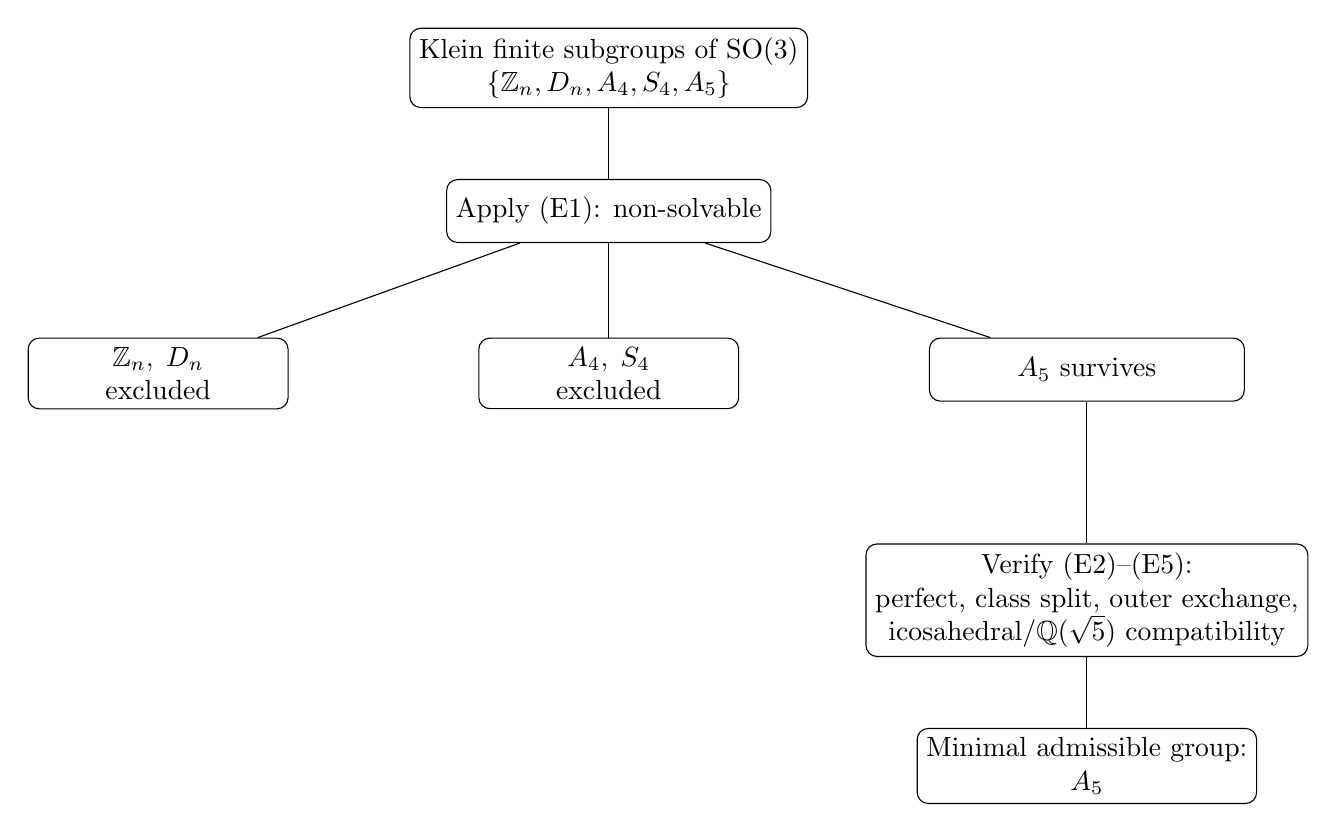
\begin{tikzpicture}[
  >=Stealth,
  node distance=9mm and 12mm,
  box/.style={draw, rounded corners, align=center, minimum width=40mm, minimum height=8mm},
  note/.style={draw, rounded corners, align=center, minimum width=33mm, minimum height=8mm},
  every edge/.style={draw, ->, thick}
]
  \node[box] (klein) {Klein finite subgroups of $\SO(3)$\\$\{\mathbb{Z}_n, D_n, A_4, S_4, A_5\}$};
  \node[box, below=of klein] (e1) {Apply (E1): non-solvable};
  \node[note, below left=12mm and 20mm of e1] (drop1) {$\mathbb{Z}_n,\;D_n$\\excluded};
  \node[note, below=12mm of e1] (drop2) {$A_4,\;S_4$\\excluded};
  \node[box, below right=12mm and 20mm of e1] (a5) {$A_5$ survives};
  \node[box, below=18mm of a5] (verify)
    {Verify (E2)--(E5):\\perfect, class split, outer exchange,\\icosahedral/$\Qsqrt$ compatibility};
  \node[box, below=of verify] (final)
    {Minimal admissible group:\\\textbf{$A_5$}};
  \draw (klein) -- (e1);
  \draw (e1) -- (drop1);
  \draw (e1) -- (drop2);
  \draw (e1) -- (a5);
  \draw (a5) -- (verify);
  \draw (verify) -- (final);
\end{tikzpicture}
\caption{Screening of Klein's finite rotation groups under the eligibility conditions
(E1)--(E5). The group $A_5$ is not postulated at the outset; it emerges as the minimal
admissible candidate.}
\label{fig:minimality-screening}
\end{figure}

%%------------------------------------------------------------
\subsubsection{The \texorpdfstring{$\Qsqrt$}{Q(sqrt5)} number field:
an algebraic structure specific to \texorpdfstring{$A_5$}{A5}}
\label{sssec:qsqrt5}
%%------------------------------------------------------------

The deeper role of $A_5$ in this construction goes beyond merely being
``the only group satisfying the selection conditions.'' The crucial
point is the following:

\begin{quote}
  \textit{The geometry of the icosahedron and the representation theory
  of $A_5$ are both governed by the same number field $\Qsqrt$.}
\end{quote}

Specifically:
\begin{itemize}
  \item \textit{Geometric side:} The edge-to-diagonal ratio of the
    regular icosahedron equals the golden ratio
    $\varphi = (1+\sqrt{5})/2 \in \Qsqrt$.
  \item \textit{Representation-theoretic side:}
    $\chi_{\rho_3}(C_5^+) - \chi_{\rho_3}(C_5^-) = \sqrt{5} \in \Qsqrt$.
\end{itemize}
By contrast, the other finite rotation groups have character fields
$\mathbb{Q}$ (for $A_4$ and $S_4$) or $\mathbb{Q}(\sqrt{-7})$ (for
$\mathrm{PSL}(2,7)$), which are unrelated to the geometric constants of
the regular polyhedra.

This number-field agreement is the algebraic root of the structure that
simultaneously produces $\sqrt{5}$, $\varphi$, and the Fibonacci
numbers. Within the discrete gauge structure selected once the Finite Readout
Principle yields finite operational holonomy and the no-go theorem
forces a discrete implementation, $A_5$ is selected, and the
coincidence of geometry and representation theory at the level of the
number field algebraically constrains the cosmological scale (as a
conditional application example).

\begin{figure}[t]
\centering
\tikzset{
  rbox/.style={draw=#1, fill=#1!12, rounded corners=7pt, line width=1.4pt,
               inner sep=8pt, align=center, font=\small},
  fieldbox/.style={draw=cField, fill=cField!15, rounded corners=10pt, line width=2.2pt,
                   minimum width=3.8cm, minimum height=1.3cm,
                   inner sep=8pt, align=center, font=\normalsize\bfseries,
                   blur shadow={shadow blur steps=5, shadow xshift=1.5pt,
                                shadow yshift=-1.5pt, shadow blur radius=4pt,
                                shadow opacity=25}},
  srcbox/.style={draw=#1, fill=#1!13, rounded corners=8pt, line width=1.6pt,
                 minimum width=3.2cm, minimum height=1.8cm,
                 inner sep=8pt, align=center, font=\small,
                 blur shadow={shadow blur steps=4, shadow xshift=1pt,
                              shadow yshift=-1pt, shadow blur radius=3pt,
                              shadow opacity=20}},
  midbox/.style={draw=#1, fill=#1!10, rounded corners=6pt, line width=1.2pt,
                 minimum width=3.6cm, minimum height=1.2cm,
                 inner sep=7pt, align=center, font=\small},
  finalbox/.style={draw=cEta, fill=cEta!18, rounded corners=9pt, line width=2.2pt,
                   minimum width=9.0cm, minimum height=1.6cm,
                   inner sep=8pt, align=center, font=\small\bfseries,
                   blur shadow={shadow blur steps=5, shadow xshift=1.5pt,
                                shadow yshift=-1.5pt, shadow blur radius=4pt,
                                shadow opacity=30}},
  mainArr/.style={draw=cArrow, line width=1.8pt,
                  -{Stealth[length=9pt, width=6pt]},
                  shorten >=2pt, shorten <=2pt},
  srcArr/.style={draw=#1, line width=1.6pt,
                 -{Stealth[length=8pt, width=5pt]},
                 shorten >=2pt, shorten <=2pt},
  labelnode/.style={draw=none, fill=white, inner sep=2pt,
                    font=\footnotesize\bfseries, text=#1},
}
\begin{tikzpicture}[node distance=1.0cm]
  %% ROW 0 — Central number field
  \node[fieldbox] (field) at (0,0)
    {Number field $\Qsqrt$\\[2pt]
     \textcolor{cField}{\footnotesize shared algebraic root}};
  %% ROW 1 — Two source pillars (narrowed horizontal offset)
  \node[srcbox=cGeo, above left=1.6cm and 0.5cm of field] (geo)
    {\textcolor{cGeo}{\textbf{Icosahedral Geometry}}\\[4pt]
     Edge-to-diagonal ratio $= \phigold$\\[2pt]
     $\phigold = \dfrac{1+\sqrt{5}}{2} \in \Qsqrt$};
  \node[srcbox=cRep, above right=1.6cm and 0.5cm of field] (rep)
    {\textcolor{cRep}{\textbf{Repr.\ Theory of $A_5$}}\\[4pt]
     Character gap $\Delta\chi = \sqrt{5}$\\[2pt]
     $\chi_{\rho_3}(C_5^+)-\chi_{\rho_3}(C_5^-)=\sqrt{5}\in\Qsqrt$};
  \draw[srcArr=cGeo] (geo.south) -- (field.north west)
    node[labelnode=cGeo, pos=0.45, xshift=-8pt] {$\phigold\in\Qsqrt$};
  \draw[srcArr=cRep] (rep.south) -- (field.north east)
    node[labelnode=cRep, pos=0.45, xshift=8pt] {$\sqrt{5}\in\Qsqrt$};
  %% ROW 2 — Derived quantities (narrowed, closer to center)
  \node[midbox=cGeo, below left=1.5cm and 0.5cm of field] (dil)
    {\textcolor{cGeo}{\textbf{Dilution factor}}\\[3pt]
     $\phigold^{-48}$\quad(vertex branch)\\[1pt]
     $N = 48 = V\cdot(|\mathrm{Stab}_v|-1)$};
  \node[midbox=cRep, below right=1.5cm and 0.5cm of field] (gap)
    {\textcolor{cRep}{\textbf{Swap-odd invariant}}\\[3pt]
     $\Delta\chi = \sqrt{5}$\\[1pt]
     (Wilson action cost gap)};
  \draw[srcArr=cGeo] (field.south west) -- (dil.north)
    node[labelnode=cGeo, pos=0.45, xshift=-10pt] {$\phigold$-branch};
  \draw[srcArr=cRep] (field.south east) -- (gap.north)
    node[labelnode=cRep, pos=0.45, xshift=10pt] {$\sqrt{5}$-branch};
  %% ROW 3 — Binet confluence (pushed well below ROW 2)
  \node[rbox=cBinet, below=4.5cm of field,
        minimum width=5.0cm, minimum height=1.5cm] (binet)
    {\textcolor{cBinet}{\textbf{Binet's Formula}}\\[3pt]
     $\sqrt{5}\cdot\phigold^{-48}
      = F_{48}^{-1}\bigl(1+\mathcal{O}(10^{-20})\bigr)$\\[2pt]
     $F_{48} = 4{,}807{,}526{,}976$};
  \draw[srcArr=cBinet] (dil.south) -- (binet.west)
    node[labelnode=cBinet, pos=0.5, xshift=-2pt, yshift=8pt] {$\phigold^{-48}$};
  \draw[srcArr=cBinet] (gap.south) -- (binet.east)
    node[labelnode=cBinet, pos=0.5, xshift=2pt, yshift=8pt] {$\sqrt{5}$};
  %% ROW 4 — Final result (further below binet)
  \node[finalbox, below=1.6cm of binet,
        minimum width=7.0cm] (eta)
    {$\etaB
      = c\,\sqrt{5}\cdot\phigold^{-48}
      = \dfrac{c}{F_{48}}\bigl(1+\mathcal{O}(10^{-20})\bigr)
      \xrightarrow{\;c=3\;}
      6.24\times10^{-10}$\\[4pt]
     \textcolor{cEta}{No free continuous parameter
       --- algebraic identity of $\Qsqrt$}};
  \draw[srcArr=cEta] (binet.south) -- (eta.north)
    node[labelnode=cEta, pos=0.45, xshift=16pt] {$\times c$\;(prefactor)};
  %% BACKGROUND PANELS
  \begin{scope}[on background layer]
    \node[draw=cGeo!30, fill=cGeo!4, rounded corners=12pt,
          fit=(geo)(dil), inner sep=8pt] {};
    \node[draw=cRep!30, fill=cRep!4, rounded corners=12pt,
          fit=(rep)(gap), inner sep=8pt] {};
  \end{scope}
  %% TITLE
  \node[font=\large\bfseries, text=black, anchor=south]
    at ([yshift=7pt] geo.north -| field)
    {$\Qsqrt$ Unification: Geometry $\times$ Repr.\ Theory $\to$ $\etaB$};
\end{tikzpicture}
\caption{Common algebraic origin of the geometric factor $\phigold$ and the
character-theoretic gap $\sqrt{5}$. Both arise from the same number field $\Qsqrt$,
which explains the appearance of the Fibonacci scale $F_{48}$ without introducing a
separate fit parameter.}
\label{fig:qsqrt-unification}
\end{figure}

%%============================================================

%%------------------------------------------------------------
\section{No-Go Theorem for Smooth-Local Finite Holonomy}
\label{sec:nogo}
%%------------------------------------------------------------

\medskip
\noindent\textit{Epistemological level:} fully [M].
Formally verified in Lean~4 with \texttt{sorry = 0}, \texttt{axiom = 0}
(\texttt{TopologyFiniteConnected.lean}, \texttt{Section7\_ContinuumNoGo.lean},
\texttt{Section7\_ContinuumDefectNoGo.lean}).
\medskip


We establish that a finite group cannot be non-trivially realised as
the connected local holonomy of a smooth connection. The argument
proceeds via the following contradiction:
\begin{enumerate}
  \item[(i)] The holonomy lies in a finite group $F$.
  \item[(ii)] The local holonomy group of a smooth connection is a
    connected Lie subgroup of $F$.
  \item[(iii)] Finite $+$ connected $+$ $T_1$ $\Rightarrow$ trivial
    group.
  \item[(iv)] Curvature $= 0$ by the Ambrose--Singer theorem~\cite{AS1953}.
  \item[(v)] Contradiction with the physical requirement of non-zero
    curvature.
\end{enumerate}

\begin{remark}[Scope of the no-go theorem]
Theorem~\ref{thm:nogo} does not exclude finite discrete gauge theories in
general.  It excludes only the interpretation of finite holonomy groups
as \emph{smooth-local} holonomy groups of smooth connections.  Finite
discrete gauge theories on continuous spacetime (e.g., Dijkgraaf--Witten
type $A_5$ gauge theories~\cite{DW1990}) lie outside the scope of this
no-go.
\end{remark}

\begin{theorem}[No-go, Theorem~3.1]
\label{thm:nogo}
Let $G$ be a finite group realised as the connected local holonomy of a
smooth connection on a smooth manifold.  Then $G$ is trivial and the
connection has zero curvature.
\end{theorem}

\begin{theorem}[Forced bifurcation, Theorem~3.2]
\label{thm:bifurcation}
Under the Finite Readout Principle, equivalently under finite
operational holonomy as given by
Proposition~\ref{prop:finite-operational-holonomy}, any non-trivial
implementation of finiteness is restricted to one of:
\begin{enumerate}
  \item[(A)] Defect/monodromy: $\rho:\pi_1(M\setminus\Sigma)\to A_5$.
  \item[(B)] Discretisation (lattice gauge theory).
\end{enumerate}
\end{theorem}

\begin{figure}[t]
\centering
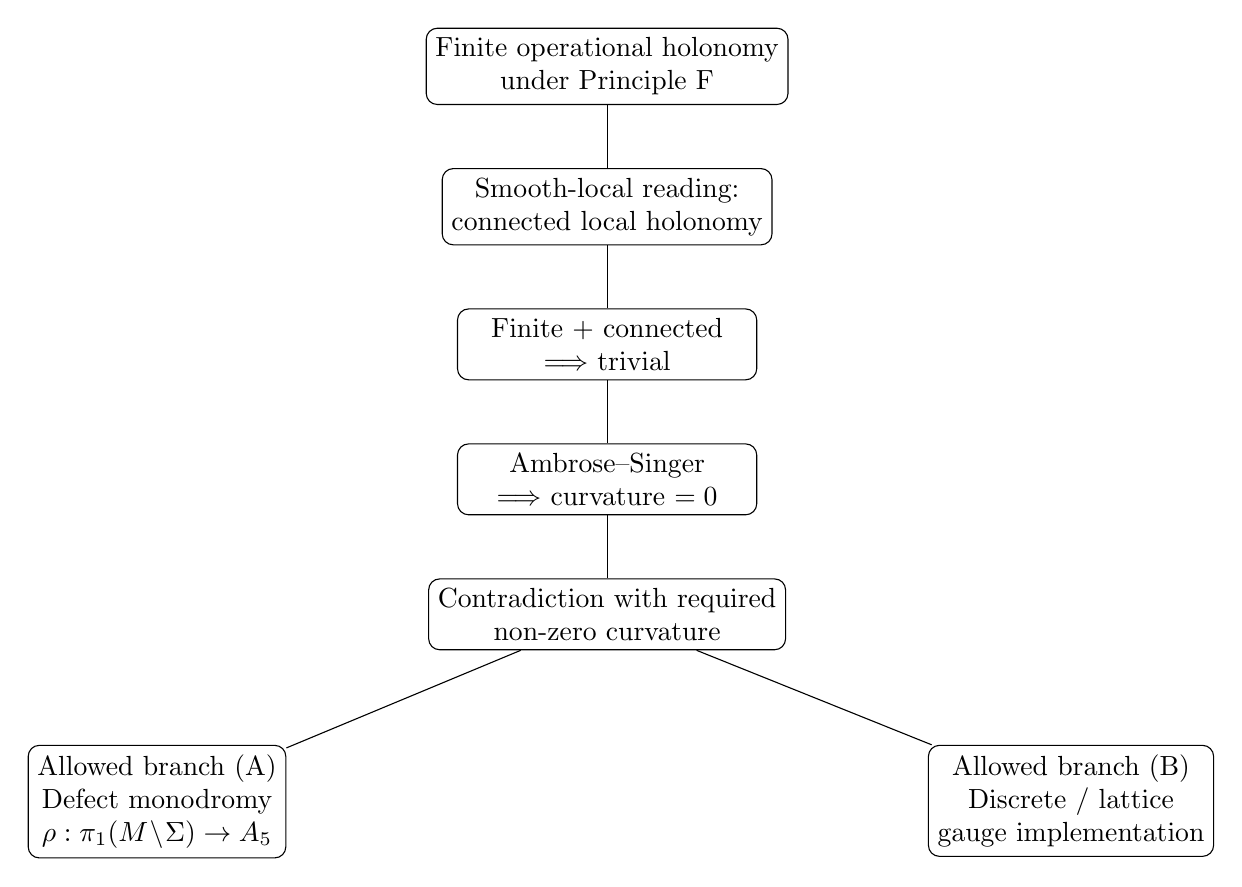
\begin{tikzpicture}[
  >=Stealth,
  node distance=8mm and 10mm,
  box/.style={draw, rounded corners, align=center, minimum width=38mm, minimum height=8mm},
  smallbox/.style={draw, rounded corners, align=center, minimum width=31mm, minimum height=8mm},
  every edge/.style={draw, ->, thick}
]
  \node[box] (start) {Finite operational holonomy\\under Principle F};
  \node[box, below=of start] (smooth) {Smooth-local reading:\\connected local holonomy};
  \node[box, below=of smooth] (trivial) {Finite + connected\\$\Longrightarrow$ trivial};
  \node[box, below=of trivial] (curv) {Ambrose--Singer\\$\Longrightarrow$ curvature $=0$};
  \node[box, below=of curv] (contra) {Contradiction with required\\non-zero curvature};
  \node[smallbox, below left=12mm and 18mm of contra] (defect)
    {Allowed branch (A)\\Defect monodromy\\$\rho:\pi_1(M\!\setminus\!\Sigma)\to A_5$};
  \node[smallbox, below right=12mm and 18mm of contra] (lattice)
    {Allowed branch (B)\\Discrete / lattice\\gauge implementation};
  \draw (start) -- (smooth);
  \draw (smooth) -- (trivial);
  \draw (trivial) -- (curv);
  \draw (curv) -- (contra);
  \draw (contra) -- (defect);
  \draw (contra) -- (lattice);
\end{tikzpicture}
\caption{Logical bifurcation forced by the no-go theorem for smooth-local finite holonomy
(Theorem~\ref{thm:bifurcation}). A smooth-local interpretation collapses to trivial holonomy
and zero curvature, so non-trivial finite holonomy must be implemented either by defect
monodromy or by a discrete/lattice gauge structure.}
\label{fig:nogo-bifurcation}
\end{figure}

\begin{theorem}[Integrative, Theorem~3.3]
\label{thm:integrative}
The following five conditions hold simultaneously: local triviality,
$\rho\neq\mathbf{1}$, and $C_5^+$ is reachable $\Rightarrow$ $C_5^-$ is
reachable by the square map.
\end{theorem}

\subsection{Structural correspondence with topological defect theory}
\label{ssec:defect}

Option~(A) is structurally analogous to cosmic strings, but differs in
four essential respects:
\begin{enumerate}
  \item $A_5$ is non-Abelian and non-solvable (the fusion rule is
    non-trivial).
  \item The $C_5^+/C_5^-$ exchange occurs only via $\mathrm{Out}(A_5)$
    (the basis for the matter/antimatter distinction).
  \item Irreversibility arises from solvable opacity (algebraic
    irreversibility, Lemma~\ref{lem:opacity}).
  \item The creation mechanism has not been established (Open
    Problem~G1').
\end{enumerate}



%%============================================================
\section{Discrete Implementation: Lattice Gauge Action and Heat-Bath Dynamics}
\label{sec:lattice}

\medskip
\noindent\textit{Epistemological level:} [M] for Theorems~\ref{thm:cost-gap}--\ref{thm:flatness} (Lean~4 verified); [Model] for Section~\ref{ssec:heatbath}.
\medskip

This section develops the discrete implementation forced once the
smooth-local branch is ruled out and the operational input is taken to
be finite readout, equivalently finite operational holonomy
(Section~\ref{sec:nogo}).

\subsection{Wilson lattice gauge action}
\label{ssec:wilson}

We represent spacetime as a finite graph $\Gamma$ and define a
Wilson-type action:
\begin{equation}
  S[U] = \sum_{p} \left(1 - \frac{\chi(U_{\mathrm{loop}}(p))}{\chi(e)}\right).
  \label{eq:wilson}
\end{equation}
The only character that distinguishes $C_5^+$ from $C_5^-$ is
$\rho_3/\rho_3'$ (essentially unique).  Choosing $\chi = \chi_{\rho_3}$
gives the following three theorems, all verified in Lean~4.

\begin{theorem}[Cost gap, Theorem~4.1]
\label{thm:cost-gap}
$\mathrm{cost}(C_5^-) - \mathrm{cost}(C_5^+) = \sqrt{5}$.
\end{theorem}

\begin{theorem}[Uniqueness of $\sqrt{5}$ component, Theorem~4.2]
\label{thm:sqrt5-unique}
Only $C_5^\pm$ plaquettes carry a $\sqrt{5}$ component in the Wilson
cost; all other conjugacy classes have rational costs.
\end{theorem}

\begin{theorem}[Flatness, Theorem~4.3]
\label{thm:flatness}
If all plaquettes are flat, $S[U] = 0$.
\end{theorem}


\subsection{Minimal effective field theory sketch}
\label{ssec:eft}

The baryon number operator is defined by
\begin{equation}
  B(U_{\mathrm{loop}}) :=
  \begin{cases}
    +1 & \text{if } U_{\mathrm{loop}} \in C_5^+, \\
    -1 & \text{if } U_{\mathrm{loop}} \in C_5^-, \\
    \phantom{+}0 & \text{otherwise,}
  \end{cases}
  \label{eq:baryon-op}
\end{equation}
and the rate asymmetry is
\begin{equation}
  \Gamma(C_5^+ \to X) - \Gamma(C_5^- \to X) \propto (a - a')\sqrt{5}.
  \label{eq:rate-asymmetry}
\end{equation}
The purpose of this sketch is not to present a complete dynamical
theory, but to demonstrate how the algebraic structure connects to the
particle-physics description.

%%------------------------------------------------------------
\subsection{Heat-bath dynamics}
\label{ssec:heatbath}
%%------------------------------------------------------------

\subsubsection{Wilson action $\to$ heat-bath $\to$ central distribution $\mu$}
\label{sssec:heatbath-central}

The heat-bath update kernel
\begin{equation}
  \mu_\beta(g) \propto \exp\!\left(-\beta\Bigl(1 - \frac{\chi(g)}{\chi(e)}\Bigr)\right)
  \label{eq:heatbath}
\end{equation}
is a class function and therefore a \emph{central} distribution,
falling naturally into the $T_\mu$ framework of
Section~\ref{ssec:model-sketch}.  This structurally closes Failure
Mode~FM2: the non-centrality objection does not arise for heat-bath
dynamics.

\subsubsection{\texorpdfstring{$\rho_3/\rho_3'$}{rho3/rho3'} alternatives
  and \texorpdfstring{$\mathbb{Z}_2$}{Z2} vacuum selection}
\label{sssec:z2-vacuum}

A $\mathbb{Z}_2$ branch of $\chi = \chi_{\rho_3}$ vs.\
$\chi = \chi_{\rho_3'}$ inevitably arises.  In the low-temperature phase
of the Ising coupling, $\sigma$ aligns, yielding $a \neq a'$ from the
vacuum selection.

\subsubsection{Reduction of \texorpdfstring{$a - a'$}{a-a'} to occupation
  difference}
\label{sssec:occupation}

\begin{equation}
  a - a' = \frac{\sqrt{5}}{3}\left(m_{C_5^+} - m_{C_5^-}\right),
  \label{eq:occupation}
\end{equation}
where $m_{C_5^\pm}$ denotes the occupation number of the respective
conjugacy-class sector.  The remaining challenge reduces to a
quantitative lattice-dynamics problem: how to generate a difference in
the occupation of $C_5^+$ and $C_5^-$.

%%============================================================
\section{Claim 1: Galois Realization Theorem}
\label{sec:claim1}
%%============================================================

\noindent\textit{Epistemological level: fully \tagM.
Formally verified in Lean~4 with \texttt{sorry} $= 0$,
\texttt{axiom} $= 0$ \textup{(}\texttt{ConjugacyClassGalois.lean},
line~430\textup{)}.}

\bigskip

%%------------------------------------------------------------
\subsection{Main theorems}
\label{ssec:claim1-main}
%%------------------------------------------------------------

\begin{theorem}[Inversion conservation]
\label{thm:inversion}
For every $g \in A_5$ with $\mathrm{ord}(g) = 5$,
\[
  g^{-1} \sim_{A_5} g.
\]
\end{theorem}

\begin{theorem}[Galois exchange]
\label{thm:galois-exchange}
The square map $g \mapsto g^2$ exchanges the two conjugacy classes
$C_5^+$ and $C_5^-$.
\end{theorem}

\begin{theorem}[Class size]
\label{thm:class-size}
$|C_5^+| = |C_5^-| = 12$.
\end{theorem}

All three theorems are verified by exhaustive traversal using
\texttt{native\_decide} in Lean~4. The indicator gap
\begin{equation}
  \Delta\chi := |\chi_{\rho_3}(C_5^+) - \chi_{\rho_3}(C_5^-)| = \sqrt{5}
  \label{eq:deltachi}
\end{equation}
is an invariant of the Galois exchange of
Theorem~\ref{thm:galois-exchange}.

\paragraph{Inversion invariance.}
By Theorem~\ref{thm:inversion}, $g^{-1}$ lies in the same conjugacy class
as $g$ for all order-$5$ elements in $A_5$. Hence the branch indicator is
inversion-invariant:
\[
B(\ell^{-1}) = B(\ell).
\]
This identity is structural and will be used repeatedly in the
baryogenesis application.

%%------------------------------------------------------------
\subsection{Proof sketch}
\label{ssec:claim1-proof}
%%------------------------------------------------------------

\paragraph{Why do 5-cycle conjugacy classes split in $A_5$?}
Let $\sigma = (0\,1\,2\,3\,4) \in A_5$.  The centralizer of $\sigma$
in $S_5$ is
\[
  Z_{S_5}(\sigma) = \langle\sigma\rangle \cong \mathbb{Z}/5\mathbb{Z},
\]
and $Z_{S_5}(\sigma) \subset A_5$ (since every power of a $5$-cycle is
an even permutation).  Hence $Z_{S_5}(\sigma) \cap (S_5\setminus A_5)
= \emptyset$, which is precisely the condition for the single $S_5$-class
of $5$-cycles to split into two $A_5$-classes
(see, e.g.,~\cite{Isaacs1994}).

\paragraph{Why does the square map swap the classes?}
The square map acts on exponents as $k \mapsto 2k \pmod{5}$.  Since
$2$ is a quadratic non-residue modulo $5$, it interchanges the
quadratic-residue set $\mathrm{QR}_5 = \{1,4\}$ and the
non-residue set $\mathrm{NR}_5 = \{2,3\}$:
\[
  1 \xmapsto{\times 2} 2, \quad
  4 \xmapsto{\times 2} 3, \quad
  2 \xmapsto{\times 2} 4, \quad
  3 \xmapsto{\times 2} 1 \pmod{5}.
\]
Table~\ref{tab:powers} tracks the conjugacy class of each power of a
representative $g \in C_5^+$.

\begin{table}[h]
\caption{Conjugacy class of powers of $g \in C_5^+$.}
\label{tab:powers}
\begin{tabular}{@{}lccccc@{}}
\toprule
Power & $g^1$ & $g^2$ & $g^3$ & $g^4 = g^{-1}$ & $g^5 = e$ \\
\midrule
Class & $C_5^+$ & $C_5^-$ & $C_5^-$ & $C_5^+$ & $\{e\}$ \\
\botrule
\end{tabular}
\end{table}

The table confirms simultaneously that $g^{-1} = g^4 \in C_5^+$
(Theorem~\ref{thm:inversion}) and that $g^2 \in C_5^-$
(Theorem~\ref{thm:galois-exchange}).
%%============================================================
\section{Claim 2: \texorpdfstring{$\mathrm{Out}(A_5)$}{Out(A5)}
  Necessity Theorem}
\label{sec:claim2}
%%============================================================

\noindent\textit{Epistemological level: fully \tagM.
Target: \texttt{sorry} $= 0$, \texttt{axiom} $= 0$ in Lean~4
\textup{(}\texttt{OutA5Necessity.lean},
\texttt{Baryon\_\allowbreak S4\_\allowbreak OutNecessity.lean}\textup{)}.}

\bigskip

%%------------------------------------------------------------
\subsection{Main lemma and theorem}
\label{ssec:claim2-main}
%%------------------------------------------------------------

\begin{lemma}[Inner automorphisms preserve $C_5^+$]
\label{lem:inner-preserve}
Every inner automorphism of $A_5$ preserves each conjugacy class.  In
particular, no element of $\mathrm{Inn}(A_5)$ exchanges $C_5^+$ and
$C_5^-$.
\end{lemma}

\begin{proof}
Immediate from the definition of conjugacy classes: for any $\phi_h \in
\mathrm{Inn}(A_5)$ defined by $\phi_h(g) = hgh^{-1}$, we have
$\phi_h(C_5^+) = C_5^+$ by definition of the conjugacy class.
\end{proof}

\begin{theorem}[$\mathrm{Out}(A_5)$ necessity]
\label{thm:out-necessity}
\leavevmode
\begin{enumerate}
  \item[(a)] The transposition $\tau = (0\,1) \in S_5 \setminus A_5$
    exchanges $C_5^+ \leftrightarrow C_5^-$ via conjugation.
  \item[(b)] This exchange cannot be achieved by any element of $A_5$
    \textup{(}Lemma~\ref{lem:inner-preserve}\textup{)}.
  \item[(c)] The exchange $C_5^+ \leftrightarrow C_5^-$ is realised
    exclusively by non-trivial elements of
    $\mathrm{Out}(A_5) \cong \mathbb{Z}_2$.
\end{enumerate}
\end{theorem}

\begin{proof}
Part~(a): Conjugation by $\tau = (0\,1)$ acts on the exponent $k$ of
a generator $g^k$ of a $5$-cycle by $k \mapsto k^{-1} \pmod{5}$.  Since
$\mathrm{QR}_5 = \{1,4\}$ and $\mathrm{NR}_5 = \{2,3\}$ (see
Section~\ref{sssec:axes}), this maps $C_5^+ \mapsto C_5^-$ and vice
versa.  Part~(b) follows from Lemma~\ref{lem:inner-preserve}.
Part~(c): Since $\mathrm{Aut}(A_5) \cong S_5$ and
$\mathrm{Inn}(A_5) \cong A_5$, the non-trivial coset in
$\mathrm{Out}(A_5) = \mathrm{Aut}(A_5)/\mathrm{Inn}(A_5) \cong
\mathbb{Z}_2$ is represented precisely by conjugation by elements of
$S_5 \setminus A_5$, which are all odd permutations.  Part~(a) shows
that these do exchange $C_5^\pm$, while part~(b) shows that the trivial
coset does not.
\end{proof}

\begin{figure}[t]
\centering
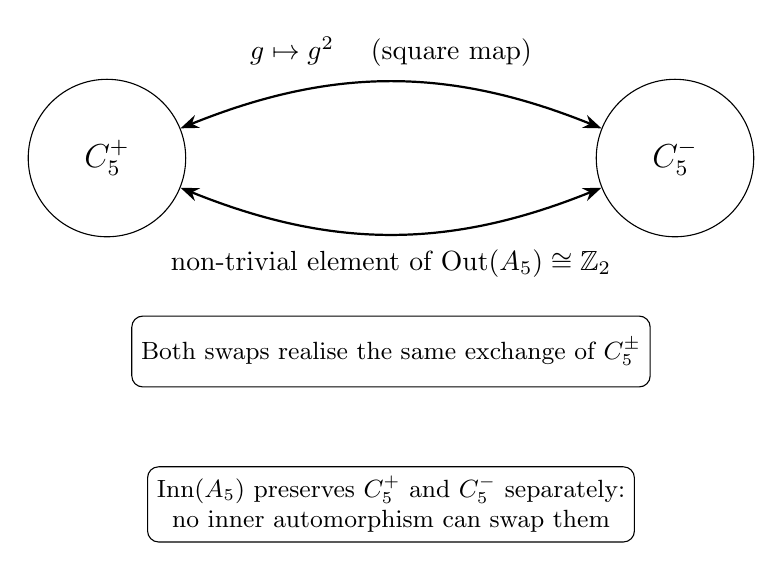
\begin{tikzpicture}[
  >=Stealth,
  node distance=30mm,
  class/.style={draw, circle, minimum size=20mm, align=center, font=\large},
  note/.style={draw, rounded corners, align=center, minimum width=52mm,
               minimum height=9mm, font=\small},
  every edge/.style={thick}
]
  \node[class] (plus)  {$C_5^+$};
  \node[class, right=52mm of plus] (minus) {$C_5^-$};
  %% Bidirectional: square map (above)
  \draw[<->, thick, bend left=22]
    (plus) to node[above=2pt] {$g\mapsto g^2$ \quad (square map)} (minus);
  %% Bidirectional: outer automorphism (below, between the circles)
  \draw[<->, thick, bend right=22]
    (plus) to node[below=2pt] {non-trivial element of $\mathrm{Out}(A_5)\cong\mathbb{Z}_2$} (minus);
  %% Notes below
  \node[note, below=20mm of $(plus)!0.5!(minus)$] (out)
    {Both swaps realise the same exchange of $C_5^\pm$};
  \node[note, below=10mm of out] (inn)
    {$\mathrm{Inn}(A_5)$ preserves $C_5^+$ and $C_5^-$ separately:\\no inner automorphism can swap them};
\end{tikzpicture}
\caption{Exchange structure of the split order-5 classes. The square map exchanges
$C_5^+$ and $C_5^-$, the same swap is realised by non-trivial elements of
$\mathrm{Out}(A_5)$, and no inner automorphism can achieve this exchange.}
\label{fig:c5-exchange}
\end{figure}

%%------------------------------------------------------------
\subsection{Structural correspondence with the Sakharov conditions}
\label{ssec:sakharov}
%%------------------------------------------------------------

We collect the three mathematical facts that underpin the structural
analogy with the Sakharov conditions~\cite{Sakharov1967}.

\paragraph{Mathematical facts (\tagM).}
\begin{itemize}
  \item[(M1)] $A_5^{\mathrm{ab}} = \{e\}$: no conserved charge
    expressible as a homomorphism $A_5 \to \mathbb{Z}$ can be defined.
  \item[(M2)] $\mathrm{Out}(A_5) \cong \mathbb{Z}_2$ exchanges
    $C_5^+ \leftrightarrow C_5^-$; this exchange is impossible within
    $\mathrm{Inn}(A_5)$ (Theorem~\ref{thm:out-necessity}).
  \item[(M3)] $A_5$ is non-solvable: every solvable-group probe
    trivialises (``opacity''), accumulating a $60^N$ degeneracy
    over $N$ stages.
\end{itemize}

\begin{lemma}[Opacity $\Rightarrow$ detailed-balance violation]
\label{lem:opacity}
A transition kernel in which all states collapse to a single output
breaks detailed balance for every non-degenerate stationary
distribution.
\end{lemma}

Table~\ref{tab:sakharov} displays the structural correspondence between
the Sakharov conditions and the $A_5$ mathematical facts.  The
physical responses in the right two columns depend on layer~\tagP\ and
bridge hypothesis~B2; they are analogies, not derivations.

\begin{table}[h]
\caption{Structural correspondence between Sakharov conditions and
$A_5$ mathematical facts.  The physical responses depend on
Bridge Hypothesis~B2 (\tagP).}
\label{tab:sakharov}
\begin{tabular}{@{}p{2.8cm}p{2.8cm}p{3.6cm}p{2.4cm}@{}}
\toprule
Sakharov condition &
$A_5$ mathematical fact (\tagM) &
Physical response (\tagP, via B2) &
Nature of response \\
\midrule
(S1) Baryon non-conservation &
(M1) $A_5^{\mathrm{ab}}=\{e\}$ &
Conserved baryonic charge cannot be defined &
Necessary condition for construction \\[4pt]
(S2) C/CP violation &
(M2) $\mathrm{Out}\cong\mathbb{Z}_2$ &
Matter/antimatter swap-odd asymmetry (no complex phase) &
Algebraic analogy \\[4pt]
(S3) Non-equilibrium &
(M3) Opacity + Lemma~\ref{lem:opacity} &
Detailed balance broken &
Additional source of irreversibility \\
\botrule
\end{tabular}
\end{table}

\paragraph{Limitations of the correspondence.}
\begin{itemize}
  \item (S1): $A_5^{\mathrm{ab}} = \{e\}$ is not identical to the
    dynamical non-conservation of physical baryon number; it is a
    structural algebraic statement.
  \item (S2): All irreducible representations of $A_5$ are real, so no
    CKM-type complex phase is generated (Limitation~L2).  The
    asymmetry considered here is swap-odd rather than phase-odd.
  \item (S3): The opacity argument does not claim equivalence to the
    standard out-of-equilibrium condition; it provides an additional
    source of irreversibility.
\end{itemize}

%%------------------------------------------------------------
\subsection{Definition of swap-odd asymmetry}
\label{ssec:swap-odd}
%%------------------------------------------------------------

All irreducible representations of $A_5$ are real-valued, so $A_5$
does not generate complex CP topology.  In this paper we focus instead
on the discrete topology induced by $\mathrm{Out}(A_5) \cong
\mathbb{Z}_2$.

\begin{definition}[Swap-odd asymmetry]
\label{def:swap-odd}
A quantity $Q(X)$ is \emph{swap-odd} if it changes sign under the
exchange $C_5^+ \leftrightarrow C_5^-$ effected by the non-trivial
element of $\mathrm{Out}(A_5)$.  The \emph{matter--antimatter exchange
asymmetry} is defined as the swap-odd component of the decay-rate
difference
\[
  \Gamma(C_5^+ \to X) - \Gamma(C_5^- \to X).
\]
The term ``CP violation'' is not used in this paper.
\end{definition}

Under Bridge Hypothesis~B3, the swap-odd component is one-dimensional
over $\Qsqrt$, so
\begin{equation}
  \Gamma(C_5^+ \to X) - \Gamma(C_5^- \to X) = \kappa_X \cdot \sqrt{5},
  \label{eq:swap-odd}
\end{equation}
where $\kappa_X \in \mathbb{Q}(\varphi)$ depends on the final state
$X$.  The modulus of the asymmetry always takes the form
$|\kappa_X|\sqrt{5}$, with $\sqrt{5}$ tracing back to the indicator gap
$\Delta\chi$ of equation~\eqref{eq:deltachi}.
%%============================================================
\section{Application Example: Conditional Construction of
  \texorpdfstring{$\etaB$}{etaB}}
\label{sec:application}
%%============================================================

\noindent\textit{Epistemological levels: \tagP\ $\to$ \tagE.}

\medskip\noindent
This section takes up one of the discrete-implementation branches that
the no-go theorem leaves open under the Finite Readout Principle,
equivalently under finite operational holonomy, and shows that the
algebraic structure of $A_5$ constrains the scale of $\etaB$.
A complete derivation of the dynamical mechanism is beyond the scope of
this paper (Section~\ref{ssec:limitations}, Limitation~L1;
Open Problem~G1').

%%------------------------------------------------------------
\subsection{Explicit assumptions}
\label{ssec:assumptions}
%%------------------------------------------------------------

The consequences and bridge hypotheses below are the inputs for the
application example.  They are adopted on the \emph{discretization
(lattice)} branch of the bifurcation forced by the no-go theorem, and
constitute the minimal implementation of that branch.

\subsubsection{Consequences (layer \tagM\ inherited by layer \tagP)}

\begin{description}
  \item[A1* (Uniqueness of $A_5$ holonomy).]
    Three principles --- (H1) finiteness, (H2) irreducibility, and
    (H3) completeness --- uniquely select $H \cong A_5$
    (Paper~I~\cite{PaperI}).

  \item[A4* (Solvable opacity $\Rightarrow$ $60^N$ barrier).]
    Because $A_5$ is non-solvable, every solvable probe trivialises,
    accumulating a degeneracy of $60^N$ over $N$ stages.
    Lemma~\ref{lem:opacity} prohibits detailed balance and provides a
    sufficient condition for (S3).
\end{description}

\subsubsection{Bridge hypotheses (layer \tagP)}

\begin{description}
  \item[B2 (Operational definition of matter/antimatter).]
    Matter and antimatter are defined as the doublet $(C_5^+, C_5^-)$
    exchanged by $\mathrm{Out}(A_5) \cong \mathbb{Z}_2$.  This is a
    definitional axiom; its physical content is tested post-hoc by
    verification of $R_X = \varphi^{-2}$ (Section~\ref{ssec:local-test}).

  \item[B3 (One-dimensionality and rate difference of swap-odd
    component).]
    Because the swap-odd component is one-dimensional over $\Qsqrt$,
    \begin{equation}
      \Gamma(C_5^+ \to X) - \Gamma(C_5^- \to X)
      = \kappa_X \cdot \sqrt{5}.
      \label{eq:B3}
    \end{equation}

  \item[B5 (Vertex selection principle: icosahedral dilution).]
    Since the swap-odd invariant originates from the $C_5^\pm$
    splitting, the natural localisation connecting the carrier to the
    $C_5$ sector via the shortest path is the \emph{vertex} sector.
    The residual degrees of freedom
    \begin{equation}
      48 = V \cdot (|\mathrm{Stab}_v| - 1) = 12 \times 4
      \label{eq:index48}
    \end{equation}
    give the dilution exponent, so the dilution factor is
    $\varphi^{-48}$.  Hypothesis~B5 is an explicitly falsifiable
    branch point (see Section~\ref{ssec:falsifiability}).
\end{description}

%%------------------------------------------------------------
\subsection{Three-step derivation}
\label{ssec:three-steps}
%%------------------------------------------------------------

\paragraph{Step~1: Fixing the swap-odd invariant \textup{(\tagM, \tagP\ via B3)}.}
Three independent sources converge on $\sqrt{5}$:
\begin{enumerate}
  \item The indicator gap $\Delta\chi = \sqrt{5}$
    (\tagM, equation~\eqref{eq:deltachi}).
  \item The cost difference in the Wilson lattice action is also
    $\sqrt{5}$ (Theorem~\ref{thm:cost-gap}; Lean~4 verified).
  \item Via bridge B3, the rate difference equals
    $\kappa_X \cdot \sqrt{5}$ (equation~\eqref{eq:B3}).
\end{enumerate}

\paragraph{Step~2: Dilution index \textup{(\tagP, B5)}.}
From equation~\eqref{eq:index48} the dilution factor is
$\varphi^{-48}$.

\begin{lemma}[Discrete branching, Lemma~5.2.B4]
\label{lem:discrete-branch}
The three carrier identifications yield three discrete values of the
dilution index:
\[
  N \in \{30,\;40,\;48\}
  \quad\text{(edges, faces, vertices).}
\]
The index is determined by the group action and is not continuously
adjustable.
\end{lemma}

\begin{lemma}[Minimality of carrier identification, Lemma~5.2.B5]
\label{lem:carrier-min}
Elements of order~$5$ appear only in the vertex stabiliser
$(\mathbb{Z}_5)$; all indices for $C_2$ and $C_3$ carriers are rational
integers.  Only vertex identification can produce a swap-odd component
that generates $\sqrt{5}$.
\end{lemma}

\paragraph{Step~3: Binet confluence \textup{(\tagM\ identity)}.}
Combining Steps~1 and 2 via Binet's formula
(equation~\eqref{eq:binet-48}),
\begin{equation}
  \etaB = c \cdot \sqrt{5} \cdot \varphi^{-48}
         = \frac{c}{F_{48}}\!\left(1 + O(10^{-20})\right),
  \quad F_{48} = 4{,}807{,}526{,}976.
  \label{eq:etaB}
\end{equation}
Step~3 introduces no new physical assumption; it merely ties together
the $\sqrt{5}$ of Step~1 and the $\varphi^{-48}$ of Step~2.  The
appearance of $F_{48}$ is an algebraic identity of $\Qsqrt$ and is not
a numerical coincidence.

\begin{figure}[t]
\centering
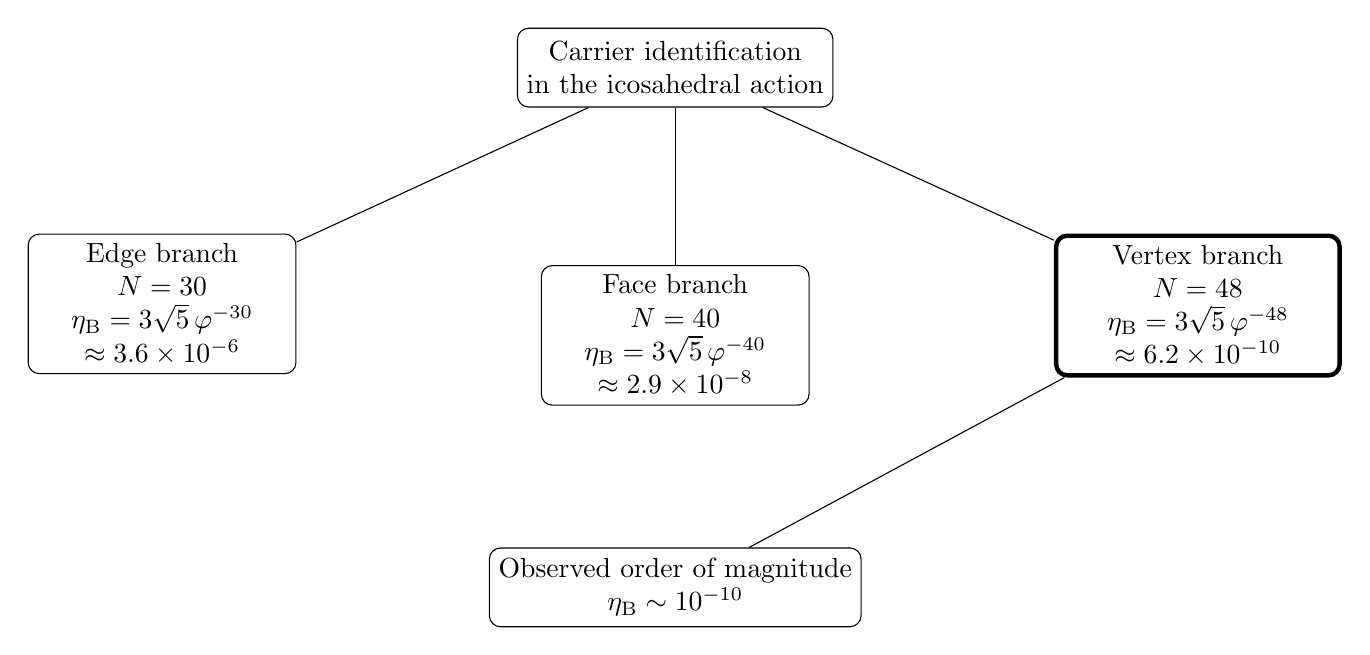
\begin{tikzpicture}[
  >=Stealth,
  node distance=10mm and 16mm,
  box/.style={draw, rounded corners, align=center, minimum width=34mm, minimum height=10mm},
  best/.style={draw, rounded corners, align=center, minimum width=36mm, minimum height=10mm, ultra thick},
  every edge/.style={draw, ->, thick}
]
  \node[box] (root) {Carrier identification\\in the icosahedral action};
  \node[box, below left=16mm and 28mm of root] (edge)
    {Edge branch\\$N=30$\\$\etaB=3\sqrt{5}\,\phigold^{-30}$\\$\approx 3.6\times10^{-6}$};
  \node[box, below=20mm of root] (face)
    {Face branch\\$N=40$\\$\etaB=3\sqrt{5}\,\phigold^{-40}$\\$\approx 2.9\times10^{-8}$};
  \node[best, below right=16mm and 28mm of root] (vertex)
    {Vertex branch\\$N=48$\\$\etaB=3\sqrt{5}\,\phigold^{-48}$\\$\approx 6.2\times10^{-10}$};
  \node[box, below=18mm of face] (obs)
    {Observed order of magnitude\\$\etaB\sim 10^{-10}$};
  \draw (root) -- (edge);
  \draw (root) -- (face);
  \draw (root) -- (vertex);
  \draw (vertex) -- (obs);
\end{tikzpicture}
\caption{Discrete compression of the baryogenesis scale into three branches determined by
icosahedral carrier identification. The vertex branch ($N=48$) selects the observed order
of magnitude.}
\label{fig:three-branches}
\end{figure}

%%------------------------------------------------------------
\subsection{Prefactor \texorpdfstring{$c$}{c}}
\label{ssec:prefactor}
%%------------------------------------------------------------

The strong-form bound $c = O(1)$ determines $\etaB \sim 10^{-10}$.
Two independent discrete principles select $c = 3$:
\begin{enumerate}
  \item[(I)] $N_c = 3$ (QCD colour number).
  \item[(II)] $|\mathrm{Stab}_{\mathrm{face}}| = 3$
    (icosahedral face-stabiliser order).
\end{enumerate}

Table~\ref{tab:prefactor} lists $\etaB$ for $c = 1,\ldots,5$ and the
deviation from the Planck~2018 CMB value
$\eta_B^{\mathrm{CMB}} \simeq 6.12\times10^{-10}$ (converted from
$\Omega_b h^2$ via $10^{10}\eta = 274\,\Omega_b h^2$~\cite{Planck2018,PDG2022}).

\begin{table}[h]
\caption{Predicted $\etaB$ for $N=48$ and $c=1,\ldots,5$.}
\label{tab:prefactor}
\begin{tabular}{@{}cccc@{}}
\toprule
$c$ & Prior principle & $\etaB$ & Deviation from Planck \\
\midrule
1 & Minimum & $2.08\times10^{-10}$ & $-66\%$ \\
2 & Euler scalar & $4.16\times10^{-10}$ & $-32\%$ \\
3 & $N_c$ or $|\mathrm{Stab}_{\mathrm{face}}|$ &
  $6.24\times10^{-10}$ & $+2\%$ \\
4 & $\dim\rho_4$ & $8.32\times10^{-10}$ & $+36\%$ \\
5 & $|\mathrm{Stab}_v|$ & $1.04\times10^{-9}$ & $+70\%$ \\
\botrule
\end{tabular}
\end{table}

Only $c=3$ falls within $5\%$ of the Planck central value.  A
first-principles derivation of $c$ is Open Problem~G12.

The role of the present construction is to constrain $\eta_B$ to a small
discrete family rather than to derive a unique numerical prefactor from
full microphysics. For that reason the coefficient is written as the
basic discrete parameter $c$, not as a composite expression. Among the
admissible small integers, $c=3$ is singled out by two independent
principles: the QCD colour number $N_c=3$ and the icosahedral face
stabiliser order $|\mathrm{Stab}_{\mathrm{face}}|=3$.

%%------------------------------------------------------------
\subsection{Why $F_{48}$ appears}
\label{ssec:binet-confluence}
%%------------------------------------------------------------

The final expression
\[
\etaB = c\sqrt{5}\,\varphi^{-48}
\]
contains two independent algebraic ingredients: the indicator gap
$\sqrt{5}$ from the split of the order-$5$ classes, and the dilution
factor $\varphi^{-48}$ from the vertex branch.

To relate this expression to an integer scale, one uses Binet's formula
\[
F_{48}=\frac{\varphi^{48}-(-\varphi)^{-48}}{\sqrt{5}}.
\]
Hence
\[
\varphi^{48}=\sqrt{5}\,F_{48}+O(\varphi^{-48}),
\qquad
\sqrt{5}\,\varphi^{-48}=F_{48}^{-1}\bigl(1+O(10^{-20})\bigr).
\]
Therefore
\[
\etaB = c\sqrt{5}\,\varphi^{-48}
     = \frac{c}{F_{48}}\bigl(1+O(10^{-20})\bigr).
\]

Step~3 introduces no new physical assumption. It only combines the
$\sqrt{5}$ factor from the Galois-theoretic indicator gap with the
dilution exponent $48$ selected by the vertex branch. The appearance of
$F_{48}$ is therefore not a separate assumption and not a numerical
coincidence; it is an algebraic consequence of the common
$\mathbf{Q}(\sqrt{5})$ structure underlying both ingredients.

%%------------------------------------------------------------
\subsection{Multiple derivations of index 48}
\label{ssec:index-48}
%%------------------------------------------------------------

The index $N = 48$ has at least two independent group-theoretic
derivations:
\begin{enumerate}
  \item \textit{Stabiliser action:}
    $48 = V \cdot (|\mathrm{Stab}_v| - 1) = 12 \times 4$
    (equation~\eqref{eq:index48}).
  \item \textit{Spectral count:}
    The number of transfer-operator independent modes for $A_5$ acting
    on the vertex set is $48$.
\end{enumerate}
The convergence of these two paths on the same integer $48$ is a
non-trivial consistency check of the vertex-branch selection.

%%------------------------------------------------------------
\subsection{Minimal model sketch: why \texorpdfstring{$\varphi$}{phi}
  and \texorpdfstring{$\sqrt{5}$}{sqrt5} enter the rate difference}
\label{ssec:model-sketch}
%%------------------------------------------------------------

Consider the convolution operator $T_\mu$ by a central probability
distribution $\mu$ on $A_5$.  By Schur's lemma, $T_\mu$ acts as scalar
multiplication on each irreducible representation.  Inspecting the
character table (Table~\ref{tab:characters}), only $\rho_3$ and
$\rho_3'$ distinguish $C_5^+$ from $C_5^-$.

Writing $a = \hat\mu(\rho_3)$ and $a' = \hat\mu(\rho_3')$, the
$C_5^\pm$ response difference is
\begin{equation}
  \Delta = (a - a')(\varphi + 1/\varphi) = (a - a')\sqrt{5}.
  \label{eq:delta-sketch}
\end{equation}
Hence for any $A_5$-invariant central distribution $\mu$, the response
difference between $C_5^+$ and $C_5^-$ takes the form $(a-a')\sqrt{5}$,
where $\sqrt{5}$ is a structure constant that inevitably emerges from
the character table.  The golden ratio $\varphi$ appears as an
eigenvalue of $T_\mu$, giving the rate ratio
\begin{equation}
  R_X = \varphi^{-2} \approx 0.382
  \label{eq:RX}
\end{equation}
in the saddle-point approximation.

\subsubsection{Falsifiability: failure-mode classification}
\label{ssec:falsifiability}

\begin{description}
  \item[FM1: $a = a'$ ($\rho_3/\rho_3'$ symmetry unbroken).]
    No asymmetry is generated; the construction fails entirely.
  \item[FM2: $\mu$ non-central.]
    The $\sqrt{5}$ fixing is outside the scope of the lattice-dynamics
    framework; addressed in Section~\ref{sssec:z2-vacuum}.
  \item[FM3: Dominant eigenvalue not from $\rho_3$.]
    The base is not $\varphi$; $R_X \neq \varphi^{-2}$.
  \item[FM4: Carrier identification changes.]
    The dilution index shifts discretely to $N \in \{30, 40\}$.
\end{description}

\subsubsection{Local prediction: independent test \texorpdfstring{$R_X$}{RX}}
\label{ssec:local-test}

The ratio
\begin{equation}
  R_X := \frac{\Gamma(C_5^+ \to X)}{\Gamma(C_5^- \to X)} = \varphi^{-2}
  \approx 0.382
  \label{eq:RX-def}
\end{equation}
depends neither on the dilution index $N$ nor on the normalisation
constant $c$.  It directly tests the $\rho_3$-dominance assumption and
is an independent fail-fast indicator.

Three observable outcomes (linking to the failure modes above):
\begin{description}
  \item[RX1 ($= $ FM1):] $R_X \simeq 1$ implies $a = a'$, showing that
    $\mathbb{Z}_2$ vacuum selection does not hold.
  \item[RX2 ($= $ FM2):] Systematic fluctuation of $R_X$ implies
    $\mu$-non-centrality, making the $\sqrt{5}$ fixing inapplicable.
  \item[RX3 ($= $ FM3):] Significant deviation of $R_X$ from
    $\varphi^{-2}$ rejects the $\rho_3$-dominance assumption.
\end{description}
%%============================================================
\section{Refutation Protocol}
\label{sec:refutation}
%%============================================================

%%------------------------------------------------------------
\subsection{Predicted vs.\ experimental values}
\label{ssec:comparison}
%%------------------------------------------------------------

Numerical comparison is not the focus of this paper (Section~\ref{ssec:three-scales}).
We first demonstrate consistency with BBN estimates, and use
CMB (Planck~2018) values as a reference estimate conditional on
$\Lambda$CDM.

\paragraph{BBN (Sch\"{o}neberg 2024~\cite{Schoneberg2024}).}
The measurement $\omega_b h^2 = 0.02218 \pm 0.00055$ (under
$\Lambda$CDM) corresponds, via the PDG conversion
$10^{10}\eta = 274\,\Omega_b h^2$~\cite{PDG2022}, to
\[
  \etaB^{\mathrm{BBN}} = (6.08 \pm 0.15)\times 10^{-10}.
\]
The $A_5$ configuration with $c=3$ gives
$\etaB = 6.2402\times10^{-10}$, a deviation of $+2.7\%$ from the BBN
central value (approximately $1.1\sigma$).

\paragraph{CMB (Planck 2018, base $\Lambda$CDM~\cite{Planck2018}).}
The directly estimated quantity is $\Omega_b h^2 \simeq
0.0224 \pm 0.0001$~\cite{Planck2018}, which translates to
\[
  \etaB^{\mathrm{CMB}} \simeq (6.12 \pm 0.04)\times 10^{-10}.
\]
The difference from our prediction is approximately $3\sigma$ on this
representation.

The frequently cited narrow error bar
$\etaB = (6.143 \pm 0.019)\times10^{-10}$ corresponds to the
(more conditional) statistical error of CMB-derived quantities; it is
not appropriate to emphasise a ``$5\sigma$ tension'' solely on this
basis. Remaining uncertainties in Planck high-polarisation modelling are
generally evaluated to be within the $0.5\sigma$ level of parameter
consistency~\cite{Planck2018lensing}.

In this paper: (i) BBN-derived estimates are the primary comparison; (ii)
CMB values serve as a $\Lambda$CDM-conditional reference.

%%------------------------------------------------------------
\subsubsection{Exhaustive evaluation of the discrete parameter space}
\label{sssec:exhaustive}
%%------------------------------------------------------------

Table~\ref{tab:exhaustive} lists all 15 combinations
$(N,c) \in \{30,40,48\}\times\{1,2,3,4,5\}$.

\begin{table}[h]
\caption{Predicted $\etaB = c\sqrt{5}\,\varphi^{-N}$ for all discrete
parameter combinations. The Planck~2018 reference value is
$\etaB^{\mathrm{CMB}} \simeq 6.12\times10^{-10}$.}
\label{tab:exhaustive}
\begin{tabular}{@{}lccccc@{}}
\toprule
Index $N$ & $c=1$ & $c=2$ & $c=3$ & $c=4$ & $c=5$ \\
\midrule
$N=30$ &
  $1.20\times10^{-6}$ & $2.40\times10^{-6}$ & $3.61\times10^{-6}$ &
  $4.81\times10^{-6}$ & $6.01\times10^{-6}$ \\
$N=40$ &
  $9.77\times10^{-9}$ & $1.95\times10^{-8}$ & $2.93\times10^{-8}$ &
  $3.91\times10^{-8}$ & $4.89\times10^{-8}$ \\
$N=48$ &
  $2.08\times10^{-10}$ & $4.16\times10^{-10}$ & $\mathbf{6.24\times10^{-10}}$ &
  $8.32\times10^{-10}$ & $1.04\times10^{-9}$ \\
\botrule
\end{tabular}
\end{table}

Of the 15 cases, only one --- $(N=48,\,c=3)$ (bold) --- falls within
$\pm 10\%$ of the Planck value. The selection of the swap-odd-invariant
carrier and the dilution exponent converges on the same
vertex/$\mathbb{Z}_5$ sector.

%%------------------------------------------------------------
\subsection{Rejection conditions}
\label{ssec:rejection}
%%------------------------------------------------------------

Table~\ref{tab:rejection} lists the conditions under which the present
construction is falsified, together with the corresponding consequence
and failure mode (FM1--FM4 defined in
Section~\ref{ssec:falsifiability}).

\begin{table}[h]
\caption{Rejection conditions for the $A_5$ baryogenesis construction.}
\label{tab:rejection}
\begin{tabular}{@{}p{3.8cm}p{4.0cm}p{2.2cm}@{}}
\toprule
Condition & Consequence & Failure mode \\
\midrule
$\etaB \not\sim 10^{-10}$ &
  Interpretation of index $48$ collapses & FM4 \\
$O(1)$ prefactor mismatch &
  The agreement is coincidental & --- \\
$R_X \neq \varphi^{-2}$ &
  $\rho_3$-dominance assumption rejected & FM3 \\
Absence of $C_5^\pm$ asymmetry &
  $a = a'$; no asymmetry generated & FM1 \\
Non-central dynamics established &
  $\sqrt{5}$ fixing inapplicable & FM2 \\
\botrule
\end{tabular}
\end{table}

%%------------------------------------------------------------
\subsubsection{Three-way branching of the \texorpdfstring{$\rho_3$}{rho3}
  dominance test (\texorpdfstring{$R_X$}{RX})}
\label{sssec:rx-branching}
%%------------------------------------------------------------

The local ratio
\[
  R_X := \frac{\Gamma(C_5^+ \to X)}{\Gamma(C_5^- \to X)} = \varphi^{-2}
\]
is an independent test that checks directly the ``kernel''
($\rho_3$~dominance) of the construction, since it does not depend on
the dilution exponent $N$ or $c_{\mathrm{norm}}$.

\begin{description}
  \item[RX1 ($=$ FM1).]
    $R_X \simeq 1$ implies $a = a'$: $\mathbb{Z}_2$ vacuum selection
    does not hold.
  \item[RX2 ($=$ FM2).]
    Systematic fluctuation of $R_X$ implies $\mu$-non-centrality,
    making the $\sqrt{5}$ fixing inapplicable.
  \item[RX3 ($=$ FM3).]
    Significant deviation of $R_X$ from $\varphi^{-2}$ rejects the
    $\rho_3$-dominance assumption.
\end{description}

%%------------------------------------------------------------
\subsection{Comparison with standard baryogenesis scenarios}
\label{ssec:comparison-standard}
%%------------------------------------------------------------

\begin{table}[h]
\caption{Comparison of baryogenesis scenarios by free-parameter count
and falsifiability.}
\label{tab:scenarios}
\begin{tabular}{@{}p{3.2cm}p{3.5cm}p{2.5cm}p{2.0cm}@{}}
\toprule
Scenario & Free parameters & $\etaB$ & Falsifiability \\
\midrule
GUT baryogenesis       & $\geq 5$ & fitting & Low \\
Electroweak baryogenesis & $\geq 3$ & fitting & Medium \\
Leptogenesis           & $\geq 4$ & fitting & Medium \\
$A_5$ (discrete constraints) &
  Discrete choices only
  ($c\in\mathbb{Z}_+$, $N\in\{30,40,48\}$) &
  ${\sim}10^{-10}$ ($c=3$, fixable in advance) &
  High \\
\botrule
\end{tabular}
\end{table}

The $A_5$ construction admits no continuously adjustable fitting
parameters; the discrete choices are exhaustively enumerated in
Table~\ref{tab:exhaustive}.

%%------------------------------------------------------------
\subsection{In-model verification: Monte Carlo test}
\label{ssec:montecarlo}
%%------------------------------------------------------------

In the discretised implementation, the heat-bath update transition count
provides a direct estimator:
\begin{equation}
  R_X = \frac{\#(C_5^+ \to X)}{\#(C_5^- \to X)}.
  \label{eq:RX-MC}
\end{equation}
A statistically significant deviation from $\varphi^{-2}$ is judged as
FM3 (rejection of $\rho_3$~dominance).  This constitutes a model-internal
consistency test that is independent of the cosmological parameters.
%%============================================================
\section{Limitations and Open Questions}
\label{sec:limitations}
%%============================================================

%%------------------------------------------------------------
\subsection{Epistemic status list}
\label{ssec:epistemic-status}
%%------------------------------------------------------------

Table~\ref{tab:epistemic} summarises the epistemic status of each
claim made in this paper, using the three-layer framework of
Section~\ref{ssec:epistemic}.

\begin{table}[h]
\caption{Epistemic status of claims. \texttt{Lean~0/0} denotes
\texttt{sorry}~$=0$, \texttt{axiom}~$=0$.}
\label{tab:epistemic}
\begin{tabular}{@{}p{6.5cm}p{5.5cm}@{}}
\toprule
Claim & Status \\
\midrule
$g\mapsto g^2$ exchanges $C_5^\pm$; $\Delta\chi=\sqrt{5}$ &
  \tagM\ Lean~4: \texttt{0/0} \\[2pt]
$\mathrm{Out}(A_5)\cong\mathbb{Z}_2$ required for the exchange &
  \tagM\ Lean~4: \texttt{0/0} target \\[2pt]
No-go: finite holonomies cannot be smooth-local &
  \tagM\ Lean~4: \texttt{0/0} \\[2pt]
Discretisation $\to$ Wilson action $\to$ $\Delta\mathrm{cost}=\sqrt{5}$ &
  \tagM\ Lean~4: \texttt{0/0} \\[2pt]
Asymmetric mode amplitude with $\sqrt{5}$ from central distribution &
  [Model] \S\ref{ssec:model-sketch} \\[2pt]
$48 = V\cdot(|\mathrm{Stab}_v|-1)$ &
  \tagM\ group action \\[2pt]
$\varphi^{-48}$ is the dilution factor &
  \tagP\ [Conditional] B5 \\[2pt]
$\etaB = c\sqrt{5}\,\varphi^{-48}\approx c/F_{48}$ &
  \tagP\tagE\ [Application, conditional] (A1*, A4*)\,+\,(B2,B3,B5) \\[2pt]
$c=3$ &
  \tagP\ fixable in advance; complete derivation [unsolved] \\[2pt]
Heat-bath centrality $\mu$; $a-a'=\tfrac{\sqrt{5}}{3}(m_+-m_-)$ &
  [Model] \S\ref{ssec:heatbath} \\[2pt]
$\mathbb{Z}_2$ vacuum selection for $a\neq a'$ &
  [Model] cosmological realisation [unsolved] \\[2pt]
Local prediction $R_X=\varphi^{-2}$ &
  [Model] \S\ref{ssec:local-test} \\
\botrule
\end{tabular}
\end{table}

%%------------------------------------------------------------
\subsection{What this paper does not claim}
\label{ssec:limitations}
%%------------------------------------------------------------

\begin{description}
  \item[(L1) Dynamical mechanism (partial).]
    Progress has been made in
    Sections~\ref{sec:nogo}--\ref{ssec:heatbath}: the no-go theorem
    rules out the smooth-local interpretation (\S\ref{sec:nogo}),
    $\sqrt{5}$ enters the Wilson action unavoidably (\S\ref{sec:lattice}),
    and heat-bath updates induce a central $\mu$, reducing $a\neq a'$ to
    $\mathbb{Z}_2$ spontaneous symmetry breaking (\S\ref{ssec:heatbath}).
    Remaining challenges are the cosmological realisation of $\mathbb{Z}_2$
    vacuum selection and a unified derivation of $\varphi^{-48}$.

  \item[(L2) Absence of complex CP phase.]
    All irreducible representations of $A_5$ are real and do not generate
    a CKM-type complex phase $\delta_{\mathrm{CP}}$.  The swap-odd
    asymmetry of this paper is a discrete asymmetry based on
    $\mathrm{Out}(A_5)\cong\mathbb{Z}_2$ and is conceptually distinct
    from the complex CP violation of the Standard Model.

  \item[(L3) Post-hoc prefactor (partial).]
    $c=3$ can be fixed in advance using the principles of
    Section~\ref{ssec:prefactor}, but a dynamical derivation has not
    been achieved.

  \item[(L4) Carrier identification (partial).]
    The minimality of vertex identification has been demonstrated
    (Lemma~\ref{lem:carrier-min}), but a dynamical argument completely
    excluding edge/face identification is still required.

  \item[(L5)] Renormalisation-group invariance of $\varphi^{-48}$
    remains unresolved.

  \item[(L6)] The dynamical meaning of $F_{48}$ remains unanswered.

  \item[(L7)] Selection rules for the pair $(\sqrt{5},\,2\log\varphi)$
    have not been established.
\end{description}

%%------------------------------------------------------------
\subsection{Open problems}
\label{ssec:open-problems}
%%------------------------------------------------------------

\begin{description}
  \item[G1' (Dynamical mechanism).]
    Cosmological realisation of $\mathbb{Z}_2$ spontaneous symmetry
    breaking; unified derivation of $\varphi^{-48}$; quantitative
    evaluation of $m_+ - m_-$.

  \item[G14 (Operational foundation of the Finite Readout Principle).]
    Provide an information-theoretic and operational derivation of the
    Finite Readout Principle, namely that finite information capacity in
    a bounded protocol implies finiteness of the operational readout
    state space $S_{\mathcal P}$, and hence finiteness of the induced
    operational holonomy image
    \[
    \operatorname{Im}\!\bigl(\rho:\pi_1(\Gamma)\to \mathrm{Sym}(S_{\mathcal P})\bigr).
    \]
    Clarify how this effective finiteness coexists with continuous
    microscopic gauge groups such as $\mathrm{SU}(2)$ and
    $\mathrm{SU}(3)$.

  \item[G15 (Wider class of discrete groups).]
    Complete assessment of whether finite subgroups of $\mathrm{SU}(2)$
    and groups of type $\mathrm{PSL}(2,p)$ can satisfy
    conditions~(E1)--(E5).
\end{description}

%%============================================================
\section{Conclusion}
\label{sec:conclusion}
%%============================================================

The main result of this paper is a no-go theorem for smooth-local finite
holonomy. A finite group cannot be realized non-trivially as the
connected local holonomy of a smooth connection: the only smooth-local
realization is the trivial one, which forces vanishing curvature.
Accordingly, any non-trivial finite holonomy framework must be
implemented through defect monodromy or through a discrete realization
such as lattice gauge structure.

The physical input used in this paper is best understood not as the
direct postulation of a finite microscopic holonomy group, but as an
operational finiteness principle: a bounded protocol with finite
resolution and finite resources can access only finitely many
operationally distinguishable readout states. From this, finite
operational holonomy follows immediately. Combined with the obstruction
theorem, this leaves a restricted finite discrete framework as the
natural setting for further construction.

Within that setting, and restricting to finite subgroups of $\SO(3)$
subject to conditions~(E1)--(E5), Klein's classification selects $A_5$
as the minimal admissible group in the present algebraic scheme. In
this precise sense, $A_5$ is not postulated as an isolated physical
dogma, but emerges as the smallest candidate compatible with the
imposed structural requirements.

The baryogenesis discussion should be read within this logical order.
The present paper does not provide a complete first-principles
microscopic derivation of $\etaB$. Rather, it shows that once the
$A_5$-based discrete framework is adopted and combined with explicit
bridge hypotheses, the candidate scale of $\etaB$ is compressed to a
small discrete family. In particular, the vertex branch selects the
observed order of magnitude $\etaB\sim10^{-10}$.

A notable structural feature is that the two key ingredients entering
the application --- the representation-theoretic gap $\sqrt{5}$ and the
geometric factor $\varphi$ --- arise from the same number field
$\Qsqrt$. This common algebraic origin explains why the final
expression may be rewritten in the form
\[
\etaB = c\sqrt{5}\,\varphi^{-48}
       = \frac{c}{F_{48}}\bigl(1+O(10^{-20})\bigr),
\]
without introducing an additional fit parameter. The appearance of
$F_{48}$ is therefore not an external numerical input, but an algebraic
consequence of the common $\Qsqrt$ structure.

What remains open is not the existence of a discrete scale constraint,
but the full operational foundation of the Finite Readout Principle,
the dynamical origin of the bridge hypotheses, the microscopic
mechanism selecting the final discrete prefactor $c$, and the explicit
construction of a physically viable defect-monodromy or lattice model
realizing the finite framework. In this sense, the paper should be read
as establishing a structural obstruction and a conditional compression
principle, rather than as claiming a completed microscopic theory.

The broader implication is that the baryogenesis problem is shifted from
one of broad continuous arbitrariness to one of sharply delimited
discrete selection. If the finite discrete framework is correct, then
the relevant question is no longer why an arbitrary small number happens
to be observed, but which discrete branch and which admissible
prefactor are physically realized.

An immediate internal test is provided by the branch-ratio prediction
$R_X=\varphi^{-2}$, which probes the $\rho_3$-dominance assumption
independently of both the dilution exponent and the normalization
constant.

%%============================================================
%% Acknowledgments + Declarations (Springer Nature mandatory)
%% ============================================================
\backmatter

\bmhead{Acknowledgments}

The formal verification in this paper is based on the Lean~4
theorem prover~\cite{Lean4} and the Mathlib mathematical
library~\cite{Mathlib}.
The author thanks the developer communities of both projects.

\bmhead{Statements and Declarations}

\paragraph{Funding.}
This research received no external funding.

\paragraph{Competing interests.}
The author declares no competing interests.

\paragraph{Ethics approval and consent to participate.}
Not applicable.

\paragraph{Consent for publication.}
Not applicable.

\paragraph{Data availability.}
No experimental data were generated or analysed in this study.
All numerical values of physical constants are taken from published
sources cited in the bibliography.
The Lean~4 source code and numerical computations supporting the
results are publicly available at
\url{https://github.com/nuu/A5_BaryonAsymmetry}
and permanently archived at Zenodo
(\url{https://doi.org/10.5281/zenodo.18958139})
under the Apache License~2.0.

\paragraph{Materials availability.}
Not applicable.

\paragraph{Code availability.}
The complete Lean~4 source code for the formal verification
(sorry\,$=$\,0, axiom\,$=$\,0) and the theorem--identifier
correspondence table are publicly available at
\url{https://github.com/nuu/A5_BaryonAsymmetry}
and permanently archived at Zenodo
(\url{https://doi.org/10.5281/zenodo.18958139})
under the Apache License 2.0.
The repository includes all files necessary to reproduce
the verification: \texttt{lakefile.lean}, Mathlib dependency
specifications, and per-section Lean source files
(\texttt{Section1\_Introduction.lean} through
\texttt{Section8\_Conclusion.lean} and auxiliary modules).

\paragraph{Author contribution.}
M.~Numagaki is the sole author and is responsible for the
conception of the theoretical framework,
all mathematical proofs and their Lean~4 formalization,
the numerical analysis, and the writing of the manuscript.

\paragraph{Use of AI-assisted tools.}
Use of Generative AI and AI-assisted technologies in the writing process
During the preparation of this work the author used ChatGPT in order to improve the readability and language of the manuscript. After using this tool/service, the author reviewed and edited the content as needed and takes full responsibility for the content of the publication.

%%============================================================
%% Appendices
%%============================================================
\begin{appendices}

%%------------------------------------------------------------
\section{Lean~4 Formalisation}
\label{app:lean}
%%------------------------------------------------------------

\subsection*{A.1\quad File list}

\paragraph{Foundation libraries.}


\vspace{6pt}
\noindent\captionof{table}{Foundation library files. All entries have
\texttt{sorry}~$=0$, \texttt{axiom}~$=0$.}
\label{tab:lean-foundation}
\begin{tabular}{@{}p{5.5cm}rp{5cm}@{}}
\toprule
File & Lines & Content \\
\midrule
\texttt{Auxiliary.lean} & 635 &
  Shared lemmas (Sylow theory and number theory toolkit) \\
\texttt{SolvabilityBelow60.lean} & 1070 &
  All groups $|G|<60$ are solvable (\S\ref{ssec:minimality}, basis for (E1)) \\
\botrule
\end{tabular}
\vspace{4pt}


\paragraph{Core theorem files.}


\vspace{6pt}
\noindent\captionof{table}{Core theorem files. All entries have
\texttt{sorry}~$=0$, \texttt{axiom}~$=0$.}
\label{tab:lean-core}
\begin{tabular}{@{}p{5.8cm}rp{4.8cm}@{}}
\toprule
File & Lines & Content \\
\midrule
\texttt{ConjugacyClassGalois.lean} & 195 &
  Claim~1: conjugacy classes and Galois swap \\
\texttt{OutA5Necessity.lean} & 498 &
  Claim~2: necessity of $\mathrm{Out}(A_5)$ \\
\texttt{TopologyFiniteConnected.lean} & 137 &
  Finite $+$ $T_1$ $+$ connected $\Rightarrow$ trivial
  (\S\ref{sec:nogo} foundation) \\
\texttt{Section7\_ContinuumNoGo.lean} & 187 &
  Sequential no-go theorem (\S\ref{sec:nogo}) \\
\texttt{Section7\_ContinuumDefectNoGo.lean} & 301 &
  Defect/monodromy enforcement $+$ $C_5^\pm$ label propagation \\
\texttt{Section7\_LatticeGaugeAction.lean} & 584 &
  Wilson lattice action $+$ $\sqrt{5}$ gap (\S\ref{sec:lattice}) \\
\texttt{Section7\_HeatBathDynamics.lean} & 573 &
  Heat-bath mechanics; $a-a'$ occupation-difference
  contraction, equation~\eqref{eq:occupation} (\S\ref{ssec:heatbath}) \\
\botrule
\end{tabular}
\vspace{4pt}


\paragraph{Section integration files.}


\vspace{6pt}
\noindent\captionof{table}{Section integration files. All entries have
\texttt{sorry}~$=0$, \texttt{axiom}~$=0$.}
\label{tab:lean-integration}
\begin{tabular}{@{}p{5.8cm}rp{5.0cm}@{}}
\toprule
File & Lines & Content \\
\midrule
\texttt{Baryon\_\allowbreak S1\_\allowbreak Introduction.lean} & 970 &
  \S1 integration: epistemological levels, Sakharov conditions,
  claims, errata \\
\texttt{Baryon\_\allowbreak S2\_\allowbreak AlgebraicPrep.lean} & 889 &
  \S2.1--\S2.5: conjugacy classes, characters, icosahedron \\
\texttt{Baryon\_\allowbreak S2\_\allowbreak MinimalityA5.lean} & 882 &
  \S2.6: Definition~\ref{def:eligible}, Theorem~\ref{thm:minimality},
  $\Qsqrt$ unification \\
\texttt{Baryon\_\allowbreak S3\_\allowbreak GaloisRealization.lean} & 731 &
  \S\ref{sec:claim1}: Claim~1 full proof (Theorems~\ref{thm:inversion}--\ref{thm:class-size}) \\
\texttt{Baryon\_\allowbreak S4\_\allowbreak OutNecessity.lean} & 531 &
  \S\ref{sec:claim2}: Claim~2 full proof and Sakharov structural correspondence \\
\texttt{Baryon\_\allowbreak S5\_\allowbreak ConditionalConstruction.lean} & 860 &
  \S\ref{sec:application}: conditional construction of $\etaB$ \\
\texttt{Baryon\_\allowbreak S6S7\_\allowbreak Refutation\allowbreak AndLimitations.lean} & 1199 &
  \S\ref{sec:refutation}--\S\ref{sec:limitations}: falsification protocol, limitations L1--L7,
  open problems G1'--G15 \\
\texttt{Baryon\_\allowbreak S8\_\allowbreak Conclusion.lean} & 814 &
  \S\ref{sec:conclusion}: integration of all claim statuses; confirmation of
  layer-\tagM\ persistence \\
\botrule
\end{tabular}
\vspace{4pt}


\noindent\textbf{Total:} 16 files, approximately 9{,}251 lines,
\texttt{sorry}~$= 0$\,/\,\texttt{axiom}~$= 0$.

\subsection*{A.2\quad Claim~1 correspondence table}


\vspace{6pt}
\noindent\captionof{table}{Lean~4 names for Claim~1 theorems.}
\label{tab:lean-claim1}
\begin{tabular}{@{}p{5.5cm}p{6cm}@{}}
\toprule
Paper theorem & Lean name \\
\midrule
Theorem~\ref{thm:inversion} & \texttt{inverse\_preserves\_conjugacy\_class} \\
Theorem~\ref{thm:galois-exchange} ($\to$) &
  \texttt{squaring\_maps\_C5plus\_to\_C5minus} \\
Theorem~\ref{thm:galois-exchange} ($\leftarrow$) &
  \texttt{squaring\_maps\_C5minus\_to\_C5plus} \\
Theorem~\ref{thm:class-size} & \texttt{C5\_class\_sizes} \\
Integration & \texttt{galois\_action\_realization} \\
\botrule
\end{tabular}
\vspace{4pt}


\subsection*{A.3\quad Claim~2 correspondence table}


\vspace{6pt}
\noindent\captionof{table}{Lean~4 names for Claim~2 theorems.}
\label{tab:lean-claim2}
\begin{tabular}{@{}p{5.5cm}p{6cm}@{}}
\toprule
Paper theorem & Lean name \\
\midrule
Lemma~\ref{lem:inner-preserve} &
  \texttt{inner\_aut\_preserves\_C5plus} \\
Theorem~\ref{thm:out-necessity}(a) ($C_5^+\to C_5^-$) &
  \texttt{odd\_perm\_maps\_C5plus\_to\_C5minus} \\
Theorem~\ref{thm:out-necessity}(a) ($C_5^-\to C_5^+$) &
  \texttt{odd\_perm\_maps\_C5minus\_to\_C5plus} \\
Theorem~\ref{thm:out-necessity}(c) &
  \texttt{tau\_not\_in\_A5} \\
Integration & \texttt{out\_A5\_necessity} \\
Lemma (power map) & \texttt{power\_map\_distribution} \\
\botrule
\end{tabular}
\vspace{4pt}


\subsection*{A.4\quad Correspondence table: \S\ref{sec:nogo} continuous no-go}


\vspace{6pt}
\noindent\captionof{table}{Lean~4 names for no-go theorem statements.}
\label{tab:lean-nogo}
\begin{tabular}{@{}p{5.5cm}p{4.5cm}p{3.5cm}@{}}
\toprule
Paper theorem & Lean name & File \\
\midrule
(iii) Finite $+$ connected $\Rightarrow$ trivial &
  \texttt{subgroup\_\allowbreak eq\_\allowbreak bot\_\allowbreak of\_\allowbreak fintype\_\allowbreak t1\_\allowbreak connected} &
  \texttt{TopologyFinite\allowbreak Connected.lean} \\
Theorem~\ref{thm:nogo} &
  \texttt{smoothLocal\_\allowbreak noGo} &
  \texttt{Section7\_ContinuumNoGo.lean} \\
Theorem~\ref{thm:bifurcation} &
  \texttt{curvature\_\allowbreak forces\_\allowbreak not\_\allowbreak local} &
  \texttt{Section7\_ContinuumNoGo.lean} \\
Defect reading consistency &
  \texttt{defect\_\allowbreak reading\_\allowbreak integrity} &
  \texttt{Section7\_Continuum\allowbreak DefectNoGo.lean} \\
No-go $\to$ defect (forced) &
  \texttt{nogo\_\allowbreak forces\_\allowbreak defect\_\allowbreak reading} &
  \texttt{Section7\_Continuum\allowbreak DefectNoGo.lean} \\
\botrule
\end{tabular}
\vspace{4pt}


\subsection*{A.5\quad Correspondence table: \S\ref{sec:lattice} lattice gauge action}


\vspace{6pt}
\noindent\captionof{table}{Lean~4 names for lattice gauge action theorems.}
\label{tab:lean-lattice}
\begin{tabular}{@{}p{5.5cm}p{6cm}@{}}
\toprule
Paper theorem & Lean name \\
\midrule
Lattice gauge action $S[U]$ &
  \texttt{LatticeGaugeAction.totalAction} \\
Theorem~\ref{thm:flatness} &
  \texttt{totalAction\_zero\_of\_allFlat} \\
Theorem~\ref{thm:cost-gap} &
  \texttt{plaquette\_cost\_gap\_is\_sqrt5} \\
Theorem~\ref{thm:sqrt5-unique} &
  \texttt{only\_C5\_produces\_irrational\_cost} \\
\botrule
\end{tabular}
\vspace{4pt}


\subsection*{A.6\quad Correspondence table: \S\ref{ssec:heatbath} heat-bath mechanics}


\vspace{6pt}
\noindent\captionof{table}{Lean~4 names for heat-bath mechanics.}
\label{tab:lean-heatbath}
\begin{tabular}{@{}p{6.5cm}p{5.0cm}@{}}
\toprule
Paper formula & Lean name \\
\midrule
Equation~\eqref{eq:occupation}:
  $a-a'=\tfrac{\sqrt{5}}{3}(m_{+}-m_{-})$ &
  \texttt{a\_sub\_a'} \\
$\varphi + 1/\varphi = \sqrt{5}$ &
  \texttt{phi\_add\_inv} \\
\botrule
\end{tabular}
\vspace{4pt}


\subsection*{A.7\quad Correspondence table: \S\ref{ssec:minimality}
  and \S\ref{sssec:qsqrt5}}


\vspace{6pt}
\noindent\captionof{table}{Lean~4 names for minimality and $\Qsqrt$ unification.
All in \texttt{Baryon\_\allowbreak S2\_\allowbreak MinimalityA5.lean}.}
\label{tab:lean-minimality}
\begin{tabular}{@{}p{5.5cm}p{6cm}@{}}
\toprule
Paper statement & Lean name \\
\midrule
Definition~\ref{def:eligible}, (E1) &
  \texttt{KleinType.satisfies\_E1} \\
Definition~\ref{def:eligible}, (E2) &
  \texttt{KleinType.satisfies\_E2} \\
Definition~\ref{def:eligible}, (E3) &
  \texttt{KleinType.satisfies\_E3} \\
Definition~\ref{def:eligible}, (E4) &
  \texttt{KleinType.satisfies\_E4} \\
Definition~\ref{def:eligible}, (E5) &
  \texttt{KleinType.satisfies\_E5} \\
Definition~\ref{def:eligible}, eligibility &
  \texttt{KleinType.isEligible} \\
Theorem~\ref{thm:minimality} &
  \texttt{theorem\_2\_6\_2\_minimality\_A5} \\
$\mathbb{Z}_n$: excluded at (E1) &
  \texttt{isEligible\_cyclic\_false} \\
$D_n$: excluded at (E1) &
  \texttt{isEligible\_dihedral\_false} \\
$A_4$: excluded at (E1) &
  \texttt{E1\_fails\_for\_A4} \\
$S_4$: excluded at (E1) &
  \texttt{E1\_fails\_for\_S4} \\
$A_5$: satisfies all conditions &
  \texttt{A5\_satisfies\_all\_conditions} \\
\S\ref{sssec:qsqrt5}: $\Qsqrt$ unification &
  \texttt{QSqrt5\_unity\_structural} \\
\S\ref{sssec:qsqrt5}: no $\varphi$ in $A_4$, $S_4$ &
  \texttt{no\_order5\_in\_A4\_or\_S4} \\
Integration & \texttt{file\_integrity\_check} \\
\botrule
\end{tabular}
\vspace{4pt}


%%------------------------------------------------------------
\section{Numerical Verification}
\label{app:numerical}
\setcounter{table}{0}%  reset → B1
%%------------------------------------------------------------


\vspace{6pt}
\noindent\captionof{table}{Key numerical values used in this paper.}
\label{tab:numerical}
\begin{tabular}{@{}p{6cm}p{5.5cm}@{}}
\toprule
Quantity & Value \\
\midrule
$\varphi = (1+\sqrt{5})/2$ & $1.6180339887\ldots$ \\
$\varphi^{48}$ & $10{,}749{,}957{,}122 \approx 1.0750\times10^{10}$ \\
$F_{48}$ & $4{,}807{,}526{,}976$ \\
$\varphi^{48}/F_{48}$ & $\sqrt{5} \approx 2.2360679\ldots$ \\
$3/F_{48}$ & $\approx 6.2402\times10^{-10}$ \\
$\etaB^{\mathrm{CMB}}$ (Planck $\to$ PDG conversion) &
  $(6.12\pm0.04)\times10^{-10}$ \\
$\etaB^{\mathrm{CMB}}$ (statistical; see \S\ref{ssec:comparison}) &
  $(6.143\pm0.019)\times10^{-10}$ \\
Deviation ($c=3$, $N=48$ vs.\ Planck central) & $+1.96\%$ \\
Deviation/$\sigma$ (vs.\ Planck central) & $\approx 3.0\sigma$ \\
\botrule
\end{tabular}
\vspace{4pt}


\clearpage
\end{appendices}

\bibliography{refs}

\end{document}
